% Elsevier CAS layout (Journal of Systems Architecture). Class files cas-dc.cls, cas-sc.cls and cas-common.sty are the
% CAS bundle v2.4 (copied from els-cas-templates/). Single-column switch: change cas-dc to cas-sc on the next line.
\def\casclass{cas-dc} % \def\casclass{cas-sc}
\documentclass[a4paper,fleqn]{\casclass}
% If the frontmatter runs over more than one page: \documentclass[a4paper,fleqn,longmktitle]{\casclass}

% The class already loads graphicx, amsmath/amssymb, booktabs, xcolor, hyperref (colorlinks) and geometry.
\usepackage[numbers,sort&compress]{natbib}
\usepackage{longtable}
\usepackage[section]{placeins}
\usepackage{tikz}
\usetikzlibrary{arrows.meta,positioning,fit,calc}
\usepackage{pgfplots}
\pgfplotsset{compat=1.18}
\usepgfplotslibrary{groupplots}
\usepackage[ruled,vlined,linesnumbered]{algorithm2e}
\usepackage{siunitx}
\usepackage[capitalise]{cleveref}

\makeatletter
\setlength{\@fptop}{0pt}    % Removes empty space above the top float on a float page
\setlength{\@fpsep}{4pt}    % Sets exact spacing between floats on a float page
\setlength{\@dblfptop}{0pt}
\setlength{\@dblfpsep}{4pt}
% Two-column layout: let long identifiers such as \texttt{forward\_secrecy} break after an underscore (text mode only;
% the character printed is unchanged), and allow a little extra interword stretch before a line overflows.
\DeclareRobustCommand{\_}{\ifmmode\nfss@text{\textunderscore}\else\textunderscore\allowbreak\fi}
\setlength{\emergencystretch}{1.5em}
\makeatother

\newcommand{\TODO}[1]{\textcolor{red}{[TODO: #1]}}
\newcommand{\todo}[1]{\textcolor{red}{[TODO: #1]}}
% Screenshot placeholder: \shot{file name without .png}{caption}{label}
\newcommand{\shot}[3]{%
  \begin{minipage}[t]{0.48\textwidth}\centering
  \IfFileExists{screenshots/#1.png}{\includegraphics[width=\linewidth]{screenshots/#1.png}}%
  {\fbox{\parbox[c][3.2cm][c]{0.9\linewidth}{\centering\footnotesize Screenshot pending:\\[2pt] {\tiny\texttt{\detokenize{#1.png}}}}}}\\[2pt]
  {\footnotesize #2}\label{#3}\end{minipage}}
% cas-common.sty prints an empty "ORCID(s):" footnote when no author has an ORCID; print it only when one is given.
\NewCommandCopy{\casprintorcid}{\printorcid}
\ExplSyntaxOn
\RenewDocumentCommand \printorcid { } { \seq_if_empty:NF \g_stm_orcid_seq { \casprintorcid } }
\ExplSyntaxOff
\crefname{algocf}{Algorithm}{Algorithms}
\Crefname{algocf}{Algorithm}{Algorithms}

\renewcommand{\topfraction}{0.9}\renewcommand{\bottomfraction}{0.8}\renewcommand{\textfraction}{0.07}
\renewcommand{\floatpagefraction}{0.6}
\renewcommand{\dbltopfraction}{0.9}\renewcommand{\dblfloatpagefraction}{0.6}
\setcounter{totalnumber}{4}\setcounter{topnumber}{3}\setcounter{bottomnumber}{2}\setcounter{dbltopnumber}{3}
% GENERATED by paper/scripts/make_tables.py
\newcommand{\AEADEst}{0.189}
\newcommand{\AEADRatio}{3.429}
\newcommand{\BitsBakmm}{1792}
\newcommand{\BitsRetryLostTwo}{2048}
\newcommand{\BitsVthree}{1248}
\newcommand{\BreakEvenAEAD}{0.0153}
\newcommand{\CostDroneBakmm}{2.47}
\newcommand{\CostDroneVthree}{1.854}
\newcommand{\CostServerAEADops}{3}
\newcommand{\CostServerBakmm}{0.44}
\newcommand{\CostServerVthree}{0.394}
\newcommand{\CostServerWithAEAD}{0.96}
\newcommand{\DomAllBetter}{3}
\newcommand{\DomAllEqual}{4}
\newcommand{\DomAllNC}{42}
\newcommand{\DomAllWorse}{0}
\newcommand{\DomBetter}{1}
\newcommand{\DomBetterScyther}{0}
\newcommand{\DomEqual}{4}
\newcommand{\DomFiveOnly}{7}
\newcommand{\DomNC}{33}
\newcommand{\DomVtwoBetter}{3}
\newcommand{\DomVtwoEqual}{1}
\newcommand{\DomVtwoNC}{3}
\newcommand{\DomVtwoWorse}{0}
\newcommand{\DomWorse}{0}
\newcommand{\DroneHashesVthree}{6}
\newcommand{\EvFail}{0}
\newcommand{\EvItems}{76}
\newcommand{\MeasCPU}{13th Gen Intel(R) Core(TM) i7-1360P}
\newcommand{\MeasCrypto}{46.0.7}
\newcommand{\MeasDroneBakmm}{0.0349}
\newcommand{\MeasDroneVthree}{0.0192}
\newcommand{\MeasPython}{3.12.0}
\newcommand{\MeasRuns}{1000}
\newcommand{\MeasServerBakmm}{0.035}
\newcommand{\MeasServerVthree}{0.0578}
\newcommand{\MeasWarmup}{50}
\newcommand{\MsgsRetryLostTwo}{5}
\newcommand{\NumBakmmBaseDNT}{18}
\newcommand{\NumBakmmBaseLemmas}{19}
\newcommand{\NumCSlemmas}{16}
\newcommand{\NumCSverified}{16}
\newcommand{\NumFlawsConditional}{4}
\newcommand{\NumFlawsConfirmed}{7}
\newcommand{\NumVthreeFalsified}{3}
\newcommand{\NumVthreeLemmas}{21}
\newcommand{\NumVthreeVerified}{18}
\newcommand{\PctBits}{30.4}
\newcommand{\PctDrone}{24.9}
\newcommand{\PctServerPrim}{10.5}
\newcommand{\PctStoreDrone}{44.8}
\newcommand{\ScyAutoNormalAutoFail}{4}
\newcommand{\ScyAutoNormalAutoOk}{8}
\newcommand{\ScyAutoNormalExplicitFail}{0}
\newcommand{\ScyAutoNormalExplicitOk}{16}
\newcommand{\ScyAutoRetryAutoFail}{11}
\newcommand{\ScyAutoRetryAutoOk}{4}
\newcommand{\ScyAutoRetryExplicitFail}{4}
\newcommand{\ScyAutoRetryExplicitOk}{12}
\newcommand{\ScyBakmmFiveSecs}{600}
\newcommand{\SecsBackwardSecrecyPaperDef}{154}
\newcommand{\SecsExecutable}{15}
\newcommand{\SecsExecutableTwoSessions}{670}
\newcommand{\SecsForwardSecrecyServer}{9}
\newcommand{\SecsPcsAfterKLeak}{622}
\newcommand{\SecsSecrecySk}{17}
\newcommand{\StoreDroneBakmm}{928}
\newcommand{\StoreDroneVthree}{512}
\newcommand{\StoreDroneVthreeMax}{832}
\newcommand{\StoreOwnBakmm}{512}
\newcommand{\StoreOwnVthree}{128}
\newcommand{\StoreServerBakmm}{672}
\newcommand{\StoreServerVthree}{1280}
\newcommand{\TestsPassed}{27}
\newcommand{\ThDrone}{0.309}
\newcommand{\ThServer}{0.055}
\newcommand{\TsencDrone}{0.018}
\newcommand{\TsencServer}{0.003}

% Shared TikZ styles: black/grey with one accent colour.
\definecolor{accent}{HTML}{1D4ED8}
\definecolor{warn}{HTML}{B91C1C}
\definecolor{lightgrey}{HTML}{E5E7EB}
\tikzset{
  party/.style={draw, rounded corners=2pt, fill=lightgrey, minimum width=1.6cm, minimum height=0.6cm, font=\small\bfseries},
  lifeline/.style={draw=black!45, thin},
  msg/.style={-{Stealth[length=2mm]}, accent, semithick},
  lost/.style={-{Stealth[length=2mm]}, warn, semithick, dashed},
  comp/.style={font=\scriptsize, align=left, text width=#1, inner sep=1pt},
  comp/.default=6.0cm,
  mlabel/.style={font=\scriptsize, above, inner sep=1.5pt},
  box/.style={draw, rounded corners=2pt, align=center, font=\small, inner sep=3pt},
}
% Message-sequence charts that stack every element below the previous one (no overlaps).
% \mscstart{left party}{right party}; \mscL[width]{text}; \mscR[width]{text};
% \mscmsg{r|l}{label}; \msclost{r|l}{label}; \mscend
\newcommand{\msclen}{12.6}
\newcommand{\mscstart}[2]{%
  \node[party] (pl) at (0,0) {#1}; \node[party] (pr) at (\msclen,0) {#2};
  \coordinate (prev) at (0,-0.4)}
\newcommand{\mscL}[2][6.2cm]{%
  \node[comp=#1, anchor=north west] (cur) at ($(prev)+(0.15,-0.12)$) {#2};
  \coordinate (prev) at (0,0 |- cur.south)}
\newcommand{\mscR}[2][6.2cm]{%
  \node[comp=#1, anchor=north east] (cur) at ($(prev)+(\msclen,0)+(-0.15,-0.12)$) {#2};
  \coordinate (prev) at (0,0 |- cur.south)}
\newcommand{\mscmsg}[2]{%
  \coordinate (m) at ($(prev)+(0,-0.5)$);
  \ifx r#1\draw[msg] (m) -- node[mlabel] {#2} ($(m)+(\msclen,0)$);\else
          \draw[msg] ($(m)+(\msclen,0)$) -- node[mlabel] {#2} (m);\fi
  \coordinate (prev) at ($(m)+(0,-0.05)$)}
\newcommand{\msclost}[2]{%
  \coordinate (m) at ($(prev)+(0,-0.5)$);
  \ifx r#1\draw[lost] (m) -- node[mlabel] {#2} ($(m)+(0.55*\msclen,0)$);\else
          \draw[lost] ($(m)+(\msclen,0)$) -- node[mlabel] {#2} ($(m)+(0.45*\msclen,0)$);\fi
  \coordinate (prev) at ($(m)+(0,-0.05)$)}
\newcommand{\mscend}{%
  \draw[lifeline] (pl.south) -- ($(0,0 |- prev)+(0,-0.25)$);
  \draw[lifeline] (pr.south) -- ($(\msclen,0 |- prev)+(0,-0.25)$)}


\begin{document}
\let\WriteBookmarks\relax

% STUB (to fill in): short title for the running head, e.g. \shorttitle{...}
\shorttitle{}
\shortauthors{A. Bagal and A.R. Kale}

\title[mode=title]{An improved authentication and key agreement scheme for the Internet of Drones, lightweight on the drone side, with forward and backward secrecy verified under a session bound}

\author[1]{Ankita Bagal}
% STUBS (to fill in, not invented): \cormark[1], \ead{<e-mail>}, ORCID as \author[1]{Ankita Bagal}[orcid=0000-0000-0000-0000],
% \credit{<CRediT roles>}
%\cormark[1]
%\ead{}
%\credit{}

\author[1]{Anand Ramdas Kale}
% STUBS (to fill in): \ead{<e-mail>}, ORCID, \credit{<CRediT roles>}
%\ead{}
%\credit{}

\affiliation[1]{organization={Department of Computer Science and Engineering, Visvesvaraya National Institute of Technology (VNIT)},
  city={Nagpur},
  postcode={440010},
  state={Maharashtra},
  country={India}}

% STUB (to fill in): corresponding author text, used with \cormark[1] above
%\cortext[1]{Corresponding author}

\begin{abstract}
In the Internet of Drones, every drone--ground-station session needs mutual authentication and a fresh key. BAKMM-IoD
(Wazid et al., 2025) claims these properties together with forward secrecy, untraceability and resistance to drone capture,
supported by a Scyther analysis. With Scyther and Tamarin we show that its published Scyther model never reaches any claim, that
the printed equations of two phases are inconsistent, that it has no forward secrecy, that the new temporary identity can be
replaced in transit, that a drone is traceable whenever a session does not complete, and, under a stated condition, that a data
record can be replayed (\NumFlawsConfirmed\ confirmed and \NumFlawsConditional\ conditional findings in our models).
We propose FSL-AKE v3: labelled hashing, authenticated encryption instead of XOR masking, erasure with one-way key evolution,
keyed one-time retry pseudonyms, key confirmation, and no timestamps. Tamarin verifies session-key secrecy, mutual
authentication, key confirmation, forward secrecy on both sides, backward secrecy (knowledge of a session key does not reveal
any earlier session key), next-identity secrecy and replay resistance, bounded to one session per drone--server pair (two for
backward secrecy), and retry unlinkability in a fixed two-drone scenario; Scyther reports a proof of correctness for the
explicit claims of the normal path; a hand
proof supports key indistinguishability. With the BAKMM-IoD paper's primitive timings, v3 lowers drone computation by
\PctDrone\%, communication by \PctBits\% and drone storage by \PctStoreDrone\%. The server stores more per drone
(\StoreServerVthree\ versus \StoreServerBakmm\ bits), and its server time is higher when the AES-GCM cost is estimated
from a desktop-measured AES-GCM/SHA-256 ratio (estimate \CostServerWithAEAD\ versus \CostServerBakmm\,ms).
\end{abstract}

% STUB (to fill in): JSA asks for 3-5 highlights of at most 85 characters each.
%\begin{highlights}
%\item
%\item
%\item
%\end{highlights}

% STUB (optional): graphical abstract
%\begin{graphicalabstract}
%\includegraphics{}
%\end{graphicalabstract}

\begin{keywords}
Internet of Drones \sep authenticated key agreement \sep forward secrecy \sep formal verification \sep Tamarin \sep Scyther
\end{keywords}

\maketitle

\section{Introduction}\label{sec:intro}

In the Internet of Drones (IoD), drones send commands, telemetry and sensor data to ground stations over open radio links,
and ground stations forward data to cloud servers. An attacker can listen to, block, replay and modify these messages, and can
capture a drone and read its memory. Every session therefore needs mutual authentication, a fresh session key, and protection
of earlier and later sessions when a device is compromised.

BAKMM-IoD \citep{wazid2025} is a recent scheme for this setting. It provides drone--server and server--cloud authenticated key
agreement based on hashing and XOR, and a blockchain phase for the data. Its authors claim, among other properties, mutual
authentication, forward secrecy, untraceability and resistance to drone capture and stolen-verifier attacks, and support the
claims with an informal analysis and a Scyther verification.

\subsection{Motivation and contribution}

We re-examined BAKMM-IoD with two automated tools, Scyther \citep{cremers2008} and Tamarin \citep{meier2013}, and found that several of these claims do not hold in our Scyther and Tamarin models
(\cref{sec:bakmm-analysis}). Following the structure of earlier improvement papers such as \citet{li2024}, this paper reports
the findings and proposes and verifies an improved scheme. Our contributions are:
\begin{enumerate}
  \item We show that the published Scyther listing of BAKMM-IoD never reaches any of its claims, that the printed equations of
        the drone--server and server--cloud phases are inconsistent, and report these and further attacks as findings
        (\NumFlawsConfirmed\ confirmed, \NumFlawsConditional\ conditional), each with a tool result and an executable control model.
  \item We propose FSL-AKE v3 (\emph{v3} below; its predecessor in this project is called v2), a three-message scheme without timestamps that replaces XOR masking by authenticated
        encryption, separates every hash by a label, erases the old key at each commit and evolves it one-way, and repairs a
        lost message with a keyed one-time pseudonym.
  \item We verify v3 with Tamarin (\NumVthreeVerified\ of \NumVthreeLemmas\ drone--server lemmas verified, bounded to one
        session per pair and two for three lemmas, the
        \NumVthreeFalsified\ remaining ones being stated limits), with Scyther, and with a hand proof in the Real-Or-Random style,
        and we compare v3 with BAKMM-IoD lemma by lemma under the same attacker.
  \item We compare cost with the BAKMM-IoD paper's own method and timings and with a desktop benchmark of both reference
        implementations, and we report every quantity, including those where v3 is higher.
\end{enumerate}

\subsection{Threat model}\label{sec:threat}
The attacker controls the network, as in the Dolev--Yao (DY) model \citep{dolev1983} that BAKMM-IoD uses: it reads, blocks,
replays, reorders and injects messages. In addition, as in the Canetti--Krawczyk (CK) adversary model \citep{canetti2001} that
BAKMM-IoD adopts (its Sec.~3.2), it may reveal, at any time unless a
property restricts it: a session key; the ephemeral values of a session; the current memory of a drone (device capture); the
server database; the server's volatile state; and the server's long-term secret. An insider at the registration authority
(RA) and a leak of the server database are covered by these reveals. Denial of service, side channels, timing, and the
consensus of the blockchain phase are out of scope. The blockchain phase and handover between ground stations are outside the
scheme we propose.

\subsection{Organisation}
\Cref{sec:prelim} gives notation and tools. \Cref{sec:review} reviews BAKMM-IoD and \cref{sec:bakmm-analysis} analyses it.
\Cref{sec:scheme} presents FSL-AKE v3, \cref{sec:security} its security analysis and \cref{sec:performance} its performance.
\Cref{sec:discussion} discusses limitations and \cref{sec:conclusion} concludes.

\section{Related work}

Authentication is one of the very important security services that can be applied in various networking domains .

The safe authentication mechanism utilizing blockchain technology was proposed by Yazdinejad et al. . Drones were designed to execute the planned deployment of the strategy in smart cities. At every stage of the process, this approach guaranteed the least amount of delays. A zone-based architecture was devised for a drone network, and a decentralized consensus mechanism tailored for remote drone use in smart cities was deployed.

Bera et al. introduced ACSUD-IoD, an innovative access control system designed to identify and thwart unwanted unmanned aerial vehicles (UAVs) within the IoD. The storing of transactional data within a private blockchain framework was enabled by the integration of a blockchain-based solution with ACSUD-IoD. This encompassed the delivery of secure, standardized data from an UAV to the ground station server. Consequently, the transactional data on the blockchain is verifiable. A formal security verification was performed utilizing the ``Automated Validation of Internet Security Protocols and Applications (AVISPA) tool'', alongside a comprehensive security evaluation. It illustrated that their method was adequately protected against several possible threats.

% Feng et al. proposed a ``cross-domain authentication protocol grounded in blockchain technology''. This system was designed to use 5G technology for diverse IoD applications. The aforementioned limits were duly acknowledged during the formulation of this plan with the aim of transcending them. Their methodology was based on a varied collection of signatures, all produced via threshold sharing. As a result, they successfully established a productive identity federation for collaborative domains.

Cho et al. developed an authentication mechanism for unmanned aerial vehicles (UAVs) to reduce security threats linked to unauthorized drones utilizing the IoD concept. Although their methodology reduced communication and computational requirements, yet their architecture was vulnerable to the ``Ephemeral Secret Leakage (ESL) attack under the CK-adversary model''. The method insufficiently protected the anonymity and untraceability of the participants. Another element that contributed to this issue was the absence of blockchain technology in their proposed strategy.

Gupta et al. presented a GaRuDa system, which might potentially denoted as the drone-based delivery system that operated on the blockchain technology. The integration of this system into the operations of Healthcare 5.0 applications was feasible. The IoT and blockchain technology were utilized in their approach to enable the swift and accurate distribution of medical supplies, which could be continuously monitored and recorded by many stakeholders. This was achieved by using a 5G-enabled Internet environment.

A pair of unique communication strategies for UAV environments were developed by Rodrigues et al. . Their scheme facilitated the establishment of a direct exchange of messages between two drones. Nevertheless, the main contractual arrangement has been altered within the framework of this strategy. In accordance with the CK-adversary concept, their scheme was not impervious to the possibility of an ESL attack. Moreover, their scheme lack support for the blockchain technology.

Ever  proposed an authentication system for IoT applications that used Elliptic Curve Cryptography (ECC). UAVs were considered to be mobile extensions of wireless sensor networks, operating within a hierarchical framework, according to their design. This particular design enabled the effective implementation of one-time user authentication for mobile sinks (UAVs), cluster chiefs, and sensor nodes. In contrast, their system was vulnerable to ``ESL attack under the CK-adversary model''. Moreover, their scheme did not ensure the maintenance and safeguarding of anonymity and untraceability. Another limitation of their scheme was absence of blockchain technology and it required more communication and computational costs.

Singh et al. examined the evolution and potential applications of the Internet of Drones. The advanced development of this technology has generated several apprehensions, among which the degree of security offered by autonomous robots has always been a prominent issue. Hence, they emphasized the most urgent security vulnerabilities and suggested that the most efficient approach to address these challenges would be to adopt state-of-the-art blockchain technology.

Xiong et al. introduced a secure collaborative computing system that implemented blockchain technology. They initially created a lightweight blockchain framework that was specifically designed for ``Unmanned Aerial Vehicle (UAV) Ad-Hoc Networks (UANET)''. Further, they introduced an improved ``Practical Byzantine Fault Tolerance (PBFT)'' consensus algorithm that was based on trust assessment.

Wang et al. introduced a mutual authentication method that was both simple and effective, and it exclusively relied on one-way hash algorithms and bitwise XOR operations. Additionally, the issue of a centralized trusted authority (TA) was mitigated by blockchain technology. The Real-or-Random model-based formal security analysis was employed. Further, an informal security proof was provided to prove the security of their proposed authentication mechanism. Further, Wang et al. introduced, ``BSIF: Blockchain-Based Secure, Interactive, and Fair Mobile Crowdsensing'' system. It was blockchain-based and was distinguished by its security, interactivity, and impartiality. These attributes were achieved through the integration of smart contracts and mobile devices. Yu et al. presented a ``Cross-domain Industrial IoT Based on Consortium Blockchain mechanism (CBDS) for the security of Industrial Internet of Things (IIoT). Further, they introduced consortium blockchain specifically to establish trust across IIoT domains.

Srinivas et al. developed an innovative authentication technique that was anonymous, lightweight, and relied on temporal credentials for Internet of Things (IoT)-based platforms. It was denoted as TCALAS. To enhance TCALAS, Ali et al. developed an improved version of TCALAS, referred to as iTCALAS for the secure communication of IoD.

Mishra et al. represented a framework for managing authentication and session keys using blockchain technology. This framework supported the integration of big data analytics capabilities for drones that operate on networks beyond 5G applications. Through a comprehensive security examination and scyther tool-based formal security verification, they have proven their scheme secured against the wide range of attacks.

In 2024, Algarni and Jan proposed a robust yet lightweight security mechanism utilizing a fuzzy extractor and the MD5 (Message Digest 5) algorithm to authenticate all IoD participants and ensure secure communication. However, the MD5 hash algorithm is widely recognized as less secure compared to more robust alternatives like the Secure Hash Algorithm (SHA-256). Consequently, the overall strength of their scheme is compromised. Moreover, their approach does not incorporate support for blockchain implementation.

Wazid et al. in 2025 developed a protocol for authentication and secure key management for internet of drone applications, the scheme is an advanced version of their protocol, with more security and efficiency.

\noindent\textit{Research gaps and novelty:} Blockchain technology offers powerful solutions to strengthen the security of the IoD environment. By enabling the creation of unique digital identities for individual drones, which are securely stored and managed on the blockchain, it helps mitigate the risk of impersonation attacks. In addition, the data coming securely from the drones to the ground station server is used for the transactions and later, the blocks formed from the authentic and genuine data from the drones are stored in the blockchain network maintained by the cloud servers. Storing data on semi-trusted cloud servers raises serious concerns about data poisoning attacks, which can significantly impact businesses and organizations by corrupting big data analytics, leading to financial losses and reputational damage. Research shows notable improvements in accuracy, recall, precision, and F1-score when data is free from poisoning attacks and is directly sourced from the blockchain. In this context, authentication among drones and other entities in the IoD environment becomes critical to ensure that genuine data is stored on the blockchain.

The literature review highlights that most existing authentication techniques for IoT and IoD environments are either inefficient in terms of communication and computation or vulnerable to various attacks. This underscores the need for a reliable and secure authenticated key agreement protocol to facilitate secure data aggregation at ground station servers in the IoD environment, with blockchain technology providing enhanced secure storage. Therefore, the objective of this work is to develop a novel and secure blockchain-based authentication and key management mechanism for IoD applications that is not only resistant to various attacks but also efficient in communication and computational costs, making it suitable for real-world practical applications.
\section{Preliminaries}\label{sec:prelim}

\subsection{Notation}
\Cref{tab:notation} lists the symbols of FSL-AKE v3 with their lengths and holders. For BAKMM-IoD we keep the paper's symbols
($TID_{DE}$, $RID_{DE}$, $TC_{DE}$, $MS$, $rs_1$, $rs_2$, $M_1$--$M_6$, $T_1$--$T_3$). The ground station $ES$ (the
ground-station server, GSS, of the BAKMM-IoD paper) is also called the \emph{server}; the cloud server is $CS$.
\begin{table*}[!htbp]
\centering
\footnotesize
\caption{Notation of FSL-AKE v3 (\texttt{spec/fsl\_ake\_v3.md}, Sec.~3).}
\label{tab:notation}
\setlength{\tabcolsep}{3pt}
\begin{tabular}{p{2.4cm}rp{6.4cm}p{3.6cm}}
\toprule
Symbol & Bits & Meaning & Held by \\
\midrule
$DE, ES, CS, RA$ & - & drone, ground-station server, cloud server, registration authority &  \\
$dev$ & 64 & device number, unique per server & ES \\
$TID$ & 160 & current temporary identity of the drone & DE; ES only as PRP index \\
$PID$ & 96 & current one-time retry pseudonym & DE; ES only as PRP index \\
$K$ & 256 & current key shared by DE and ES & DE; ES only encrypted under X\_db \\
$X_{ES}$ & 128 & server master secret, in a secure element & ES \\
$X_{idx}, X_{db}$ & 128 each & index and record keys derived from X\_ES at boot (E0) & ES (secure element) \\
$N_1, N_{1r}, N_2$ & 160 each & random nonces (first attempt, retry, server) & sender; public on the wire \\
$V_1, V_{1r}, V_2, V_3$ & 256 each & check values & public on the wire \\
$SK$ & 256 & session key & DE and ES, in volatile memory only, during the session \\
$KD$ & 128 & data key SK[0..127] & as SK \\
$R$ & 128 & one-time retry key & ES while committing (then erased); DE only when it needs it \\
$T$ & 288 & retry ticket: N2 encrypted under R & ES database \\
$\nu $ & 96 & AEAD nonce of a stored record & ES database \\
$ctr$ & 64 & data-record counter & sender and receiver \\
$dir$ & 32 & direction label of a data record & constant \\
\bottomrule
\end{tabular}
\end{table*}


\subsection{Primitives}
$H(\ell, x_1,\dots,x_n)$ is SHA-256 \citep{fips1804} over the length-prefixed concatenation of a label $\ell$ and the inputs;
each equation uses its own label, so no two equations hash the same input. $\mathrm{AEAD}_k(\nu; m; ad)$ is AES-128-GCM
\citep{nist80038d} with a 96-bit nonce and a 128-bit tag; decryption returns either the plaintext or a failure symbol when the
inputs are not authentic \citep{rfc5116}. $\mathrm{PRP}$ is deterministic AES-128 encryption used for database indices. No key-derivation function other
than the labelled hash is used, and no XOR.

\subsection{Verification tools}
\textbf{Tamarin} \citep{meier2013} (tamarin-prover 1.12.0 with Maude 3.5.1, as reported by the binaries) is a
symbolic prover for protocols with state. Properties are written as lemmas over trace actions; a lemma is \emph{verified} or
\emph{falsified} with a counterexample trace, and an \texttt{exists-trace} lemma shows that the protocol can run
(executability). Observational equivalence (\texttt{--diff}) \citep{basin2015} expresses unlinkability. We bound the number of consecutive sessions per drone--server pair where the unbounded search did not
terminate, and state the bound with every result.

\textbf{Scyther} \citep{cremers2008} (Windows build scyther-w32 v1.3.0; the binary reports its version as
v1.3.0-dirty) analyses protocols without state across runs. Claims such as \texttt{Secret}, \texttt{SKR},
\texttt{Alive}, \texttt{Weakagree}, \texttt{Niagree} (non-injective agreement, \citep{lowe1997}), \texttt{Nisynch}
(non-injective synchronisation, \citep{cremers2006}) and \texttt{Commit} are checked up to a bound on the number of runs; Scyther reports a \emph{proof of correctness} when a claim holds for any number of runs, and
\emph{no attack within bounds} otherwise.

\subsection{Real-Or-Random model}
In a Real-Or-Random (ROR) style model \citep{abdalla2005}, with hash functions modelled as random oracles
\citep{bellare1993}, the adversary interacts with protocol instances through
\textsf{Execute}, \textsf{Send}, \textsf{Reveal} and \textsf{Corrupt} queries and finally asks \textsf{Test} on a fresh
instance; it receives either the real session key or a random string and must tell which. The scheme is secure if the
advantage is negligible. We use a single \textsf{Test} query (the Find-then-Guess form) in \cref{sec:ror}.

\section{Review of BAKMM-IoD}\label{sec:review}

BAKMM-IoD \citep{wazid2025} has registration (Sec.~4.1 of the paper), drone--server authentication and key establishment
(Sec.~4.2), server--cloud key management (Sec.~4.3), dynamic drone addition (Sec.~4.4) and a blockchain phase (Sec.~4.5).

\subsection{Registration}
The RA gives each drone $DE_i$ the values $\{TID_{DE},\allowbreak RID_{DE},\allowbreak TC_{DE},\allowbreak MS\}$, where $TID_{DE}$ is a temporary identity,
$RID_{DE}$ and $TC_{DE}$ are hash values computed by the RA and $MS$ is a secret shared with the ground station $ES_j$. The
ground station stores $(TID_{DE}, RID_{DE})$ and $MS$ for each drone, and its own $RID_{ES}$, $TC_{ES}$.

\subsection{Drone--server authentication and key establishment}
\Cref{fig:bakmm} shows the phase (AKDDE1--4). The drone picks $rs_1$ and $T_1$ and sends
\begin{align*}
 A &= h(TC_{DE}\|rs_1\|MS\|T_1),\\
 M_1 &= h(RID_{DE}\|MS\|T_1)\oplus A,\\
 M_2 &= h(A\|RID_{DE}\|T_1).
\end{align*}
The ground station recovers $A$, checks $M_2$, picks $rs_2$, $T_2$ and a new temporary identity $TID^{new}$, and returns
\begin{align*}
 B &= h(RID_{ES}\|TC_{ES}\|rs_2\|MS\|T_2),\\
 M_3 &= h(RID_{DE}\|MS\|T_2)\oplus B,\\
 SK &= h(A\|B\|T_1\|T_2\|RID_{DE}\|MS),\\
 M_4 &= h(SK\|T_1\|T_2\|RID_{DE}),\\
 M_5 &= TID^{new}\oplus h(A\|RID_{DE}\|T_2).
\end{align*}
The drone recovers $B$, computes $SK$, checks $M_4$, recovers $TID^{new}$ and confirms with $M_6 = h(SK\|T_3)$; the ground
station checks $M_6$. Here $SK$ is written in the ground station's field order; the drone's printed order differs
(\cref{sec:f2}).
\begin{figure}[!htbp]
\centering
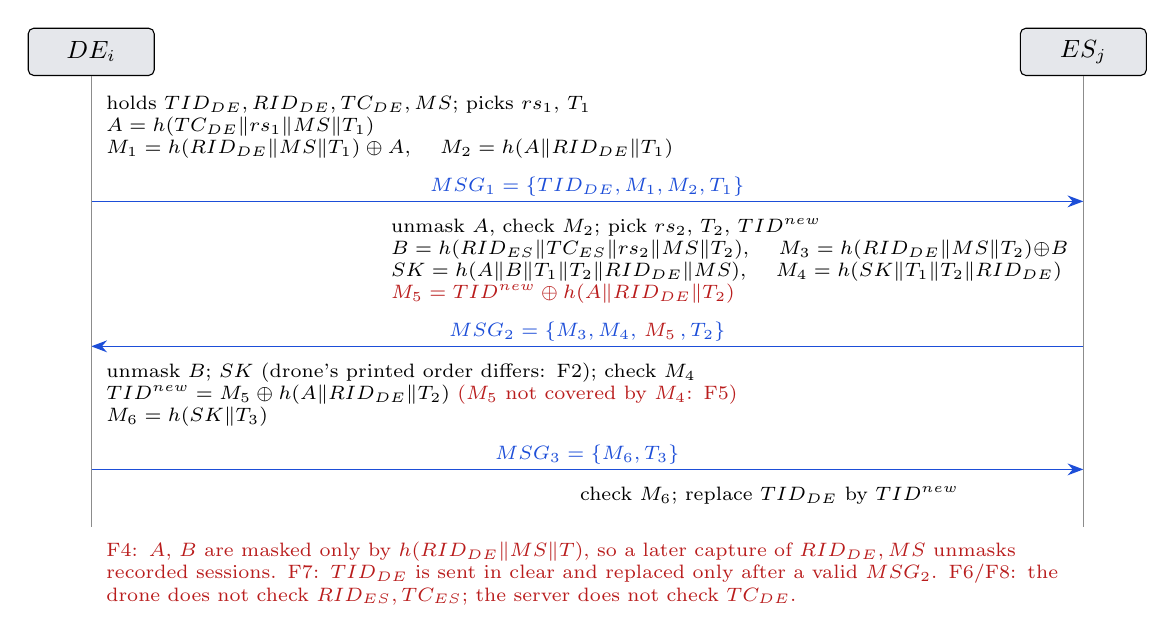
\begin{tikzpicture}
  \mscstart{$DE_i$}{$ES_j$};
  \mscL[8.0cm]{holds $TID_{DE}, RID_{DE}, TC_{DE}, MS$; picks $rs_1$, $T_1$\\
        $A = h(TC_{DE}\|rs_1\|MS\|T_1)$\\
        $M_1 = h(RID_{DE}\|MS\|T_1)\oplus A$, \quad $M_2 = h(A\|RID_{DE}\|T_1)$};
  \mscmsg{r}{$MSG_1=\{TID_{DE}, M_1, M_2, T_1\}$};
  \mscR[8.6cm]{unmask $A$, check $M_2$; pick $rs_2$, $T_2$, $TID^{new}$\\
        $B = h(RID_{ES}\|TC_{ES}\|rs_2\|MS\|T_2)$, \quad $M_3 = h(RID_{DE}\|MS\|T_2)\oplus B$\\
        $SK = h(A\|B\|T_1\|T_2\|RID_{DE}\|MS)$, \quad $M_4 = h(SK\|T_1\|T_2\|RID_{DE})$\\
        \textcolor{warn}{$M_5 = TID^{new}\oplus h(A\|RID_{DE}\|T_2)$}};
  \mscmsg{l}{$MSG_2=\{M_3, M_4, \textcolor{warn}{\boxed{\,M_5\,}}, T_2\}$};
  \mscL[8.6cm]{unmask $B$; $SK$ (drone's printed order differs: F2); check $M_4$\\
        $TID^{new} = M_5\oplus h(A\|RID_{DE}\|T_2)$ \textcolor{warn}{($M_5$ not covered by $M_4$: F5)}\\
        $M_6 = h(SK\|T_3)$};
  \mscmsg{r}{$MSG_3=\{M_6, T_3\}$};
  \mscR{check $M_6$; replace $TID_{DE}$ by $TID^{new}$};
  \mscend;
  \node[comp=12.3cm, anchor=north west, text=warn] at ($(prev)+(0.15,-0.4)$) {%
    F4: $A$, $B$ are masked only by $h(RID_{DE}\|MS\|T)$, so a later capture of $RID_{DE}, MS$ unmasks recorded sessions.
    F7: $TID_{DE}$ is sent in clear and replaced only after a valid $MSG_2$.
    F6/F8: the drone does not check $RID_{ES}, TC_{ES}$; the server does not check $TC_{DE}$.};
\end{tikzpicture}
\caption{BAKMM-IoD drone--server authentication (paper Sec.~4.2, AKDDE1--4, as modelled in our Tamarin theory).
The attacked field $M_5$ is boxed; the notes name the findings of \cref{sec:bakmm-analysis}.}
\label{fig:bakmm}
\end{figure}


\subsection{Other phases}
The server--cloud phase (AKDEC1--4) uses the same message structure between $ES_j$ and a cloud server $CS_k$. Data are sent
under the session key in the blockchain phase (BIP1--3). The paper's formal verification is a Scyther listing (its Figs.~3--4)
with results in its Fig.~5.

\section{Security analysis of BAKMM-IoD}\label{sec:bakmm-analysis}

\Cref{tab:flaws} summarises the findings. A finding is \emph{confirmed} when a tool finds the attack under the paper's own
threat model, and \emph{conditional} when it needs a stated extra condition. Every evidence pack also contains a control
model in which the same lemma or claim holds, so that a falsified result cannot come from a model that never runs.
\begin{table*}[!htbp]
\centering
\footnotesize
\caption{Findings on BAKMM-IoD. Each result comes from the pack's own model (\texttt{evidence/F1}--\texttt{F11}, files \texttt{model.spdl}/\texttt{model.spthy}), not from the shared-lemma theories of \cref{tab:tamarin,tab:tamarin-extra}; each pack also holds an executable control run.}
\label{tab:flaws}
\setlength{\tabcolsep}{3pt}
\begin{tabular}{p{0.6cm}p{1.6cm}p{4.2cm}p{5.2cm}p{2.0cm}}
\toprule
Id & Tier & Finding & Tool result (flaw run) & Tool \\
\midrule
F1 & confirmed & The paper's Scyther model gives an empty result & Scyther Reachable\_DE9: Fail; Scyther Reachable\_ES9: Fail & Scyther \\
F2 & confirmed & Printed session-key field order differs between drone and server & scyther: model as printed rejected (Scyther error) & Scyther \\
F3 & confirmed & Printed m1 and m2 use different hash inputs in the server-cloud phase & scyther: model as printed rejected (Scyther error) & Scyther \\
F4 & confirmed & No forward secrecy & Tamarin forward\_secrecy: falsified & Tamarin \\
F5 & confirmed & The new temporary identity can be replaced in transit & Scyther Niagree\_DE4: Fail; Scyther Nisynch\_DE5: Fail; Tamarin agreement\_on\_TIDnew: falsified & Scyther and Tamarin \\
F6 & confirmed & A captured drone accepts the attacker as its server & Tamarin drone\_agrees\_with\_server: falsified & Tamarin \\
F7 & confirmed & A drone is traceable whenever a session does not complete & Tamarin Observational\_equivalence: falsified & Tamarin \\
F8 & conditional & The server's table is enough to act as any of its drones & Tamarin server\_agrees\_with\_drone: falsified & Tamarin \\
F9 & conditional & With equal timestamps a listener computes the new temporary identity & Tamarin TIDnew\_secret: falsified & Tamarin \\
F10 & conditional & M1 and M3 share one mask form & Tamarin TIDnew\_secret: falsified & Tamarin \\
F11 & conditional & A data record can be delivered twice & Tamarin data\_taken\_in\_once: falsified & Tamarin \\
\bottomrule
\end{tabular}
\end{table*}


\subsection{F1: the published Scyther model never reaches its claims}\label{sec:f1}
\textbf{Paper's claim.} Sec.~6 and Fig.~5 of the paper report that all claims hold.
\textbf{Finding.} Running the published listing gives the reported \texttt{Ok} results, but Scyther's role
characterisation shows that neither role can finish (\texttt{Reachable} claims fail). Every value is declared \texttt{const}
inside each role, which Scyther treats as a fresh value per role, so no role passes its first receive and no claim is ever
reached. The \texttt{Ok} results therefore say nothing about the protocol. With the long-term values shared, both roles become
reachable (control).
\textbf{Root cause.} The listing does not let the two roles share their long-term values.

\subsection{F2: the printed session-key order differs between drone and server}\label{sec:f2}
AKDDE2 and AKDDE3 (with Table~5 of the paper) print the session key with different field orders:
\[ \text{AKDDE2: } SK = h(\dots\|T_1\|T_2\|RID_{DE}\|MS), \qquad \text{AKDDE3: } SK = h(\dots\|RID_{DE}\|T_1\|T_2\|MS). \]
As printed, the two sides compute different keys and no session completes; Scyther rejects the printed model, and the model with
one order is executable. \textbf{Root cause:} one value written twice with different field orders.

\subsection{F3: the printed $m_1$ and $m_2$ of the server--cloud phase differ}\label{sec:f3}
In AKDEC1--2, $m_1$ masks $h(TC_{ES}\|RS_1\|\dots)$ while $m_2$ is built on $h(RS_1\|TC_{ES}\|\dots)$, so the value the
cloud server unmasks never matches $m_2$ and every message is rejected. \textbf{Root cause:} as in F2.

\subsection{F4: no forward secrecy}\label{sec:f4}
\textbf{Paper's claim.} Sec.~3.2 and Proposition~5 state that the scheme supports forward secrecy.
\Cref{alg:f4} needs a recording of a finished session and, afterwards, the memory of the captured drone. Tamarin falsifies
\texttt{forward\_secrecy} on the paper's model and verifies key secrecy in the control model.
\textbf{Root cause.} Both key shares are XOR-masked only with $h(RID_{DE}\|MS\|T)$, which anyone holding the long-term values
can recompute; nothing is erased.
\begin{algorithm}[!htbp]
\caption{F4: recovering the key of a recorded session after drone capture}\label{alg:f4}
\KwIn{recorded $MSG_1=\{TID_{DE},M_1,M_2,T_1\}$, $MSG_2=\{M_3,M_4,M_5,T_2\}$; later, the captured drone's $RID_{DE}, MS$}
\KwOut{$SK$ of the recorded session}
$A \leftarrow M_1 \oplus h(RID_{DE}\|MS\|T_1)$\;
$B \leftarrow M_3 \oplus h(RID_{DE}\|MS\|T_2)$\;
$SK \leftarrow h(A\|B\|T_1\|T_2\|RID_{DE}\|MS)$\;
\Return $SK$; all data of that session can be decrypted\;
\end{algorithm}

\subsection{F5: the new temporary identity can be replaced in transit}\label{sec:f5}
\textbf{Paper's claim.} Proposition~2 and the paper's own \texttt{Niagree}/\texttt{Nisynch} claims.
Both sides complete with the same key but different temporary identities (\cref{alg:f5}). In the F5 evidence pack's own
Scyther model (\texttt{evidence/F5/model.spdl}), Scyther reports \texttt{Fail} for \texttt{Niagree}, \texttt{Nisynch} and
\texttt{Commit} on $TID^{new}$ (claims DE4, DE5, DE10), with \texttt{Ok} in the control model; in the pack's own Tamarin model
with real XOR (\texttt{evidence/F5/model.spthy}) \texttt{agreement\_on\_TIDnew} is falsified and \texttt{agreement\_on\_SK}
verified. The shared-lemma BAKMM-IoD theory of \cref{tab:tamarin}, which is larger, did not terminate on \texttt{tid\_agreement};
in the Scyther model with v3's claim set (\cref{tab:scyther}) all attack graphs on \texttt{Niagree}/\texttt{Nisynch} are this
alteration. \textbf{Root cause.} $M_4 = h(SK\|T_1\|T_2\|RID_{DE})$ does not cover $M_5$.
\begin{algorithm}[!htbp]
\caption{F5: replacing $TID^{new}$}\label{alg:f5}
\KwIn{control of the channel}
intercept $MSG_2=\{M_3,M_4,M_5,T_2\}$\;
replace $M_5$ by any value $M_5^{*}$; forward $\{M_3,M_4,M_5^{*},T_2\}$\;
the drone checks $M_4$, which does not cover $M_5$, and stores $TID^{*} = M_5^{*}\oplus h(A\|RID_{DE}\|T_2)\neq TID^{new}$\;
\end{algorithm}

\subsection{F6: a captured drone accepts the attacker as its server}\label{sec:f6}
With the drone's $RID_{DE}$ and $MS$, the attacker answers $MSG_1$ itself: it picks any $B^{*}$, sends
$M_3 = h(RID_{DE}\|MS\|T_2)\oplus B^{*}$ and the matching $M_4$, and the drone accepts a key the attacker knows without any
server. Tamarin falsifies \texttt{drone\_agrees\_with\_server}. \textbf{Root cause.} The drone does not check that the unmasked
share contains $RID_{ES}$ or $TC_{ES}$; it does not store them. (FSL-AKE v3 keeps this limit, \cref{sec:discussion}.)

\subsection{F7: a drone is traceable whenever a session does not complete}\label{sec:f7}
$TID_{DE}$ travels in clear in $MSG_1$ and is replaced only after a valid $MSG_2$. An attacker who blocks $MSG_2$ sees the same
$TID_{DE}$ in every new attempt and links them. Tamarin falsifies observational equivalence between ``same drone'' and
``two drones''; Scyther cannot express the property. \textbf{Root cause.} No identifier changes between attempts.

\subsection{Conditional findings F8--F11}\label{sec:f8}
\textbf{F8} (condition: the attacker reads the server database, which Proposition~4 excludes while Sec.~1.2 names stolen
verifiers as a risk): with $(RID_{DE}, MS)$ from the server table the attacker builds a valid $MSG_1$ and $M_6$, and the
server accepts a session the drone never ran; Tamarin falsifies \texttt{server\_agrees\_with\_drone} in the pack's own model
(\texttt{evidence/F8/model.spthy}), while the shared-lemma BAKMM-IoD theory did not terminate (\cref{tab:tamarin}). As in
\cref{tab:flaws}, all results in this section come from the packs' own models.
\textbf{F9} (condition: $T_2 = T_1$; the paper does not state the clock resolution): the mask of $M_5$ equals $M_2$, so a
listener computes $TID^{new} = M_5\oplus M_2$; Tamarin falsifies \texttt{TIDnew\_secret}.
\textbf{F10} (condition: $RID_{DE}$ leaks from an RA insider and one server key share $B$ leaks): $M_1$ and $M_3$ share the mask
form $h(RID_{DE}\|MS\|T)$, so a recovered $M_3$ mask is a valid $M_1$ mask and the attacker learns the $TID^{new}$ the server
issues; the session key is not broken; Tamarin falsifies \texttt{TIDnew\_secret}. \textbf{F11} (condition: data under the session key is plain encryption, the paper
not describing a record format): a recorded data record is accepted twice; Tamarin falsifies \texttt{data\_taken\_in\_once}.

\section{The proposed scheme: FSL-AKE v3}\label{sec:scheme}

FSL-AKE v3 is a drone--server and server--cloud authenticated key agreement with key confirmation. \Cref{tab:rationale} lists
each design change, the findings it addresses and its cost effect; the full specification is \texttt{spec/fsl\_ake\_v3.md} of
the artifact. \Cref{fig:network} shows the entities.
\begin{figure}[!htbp]
\centering
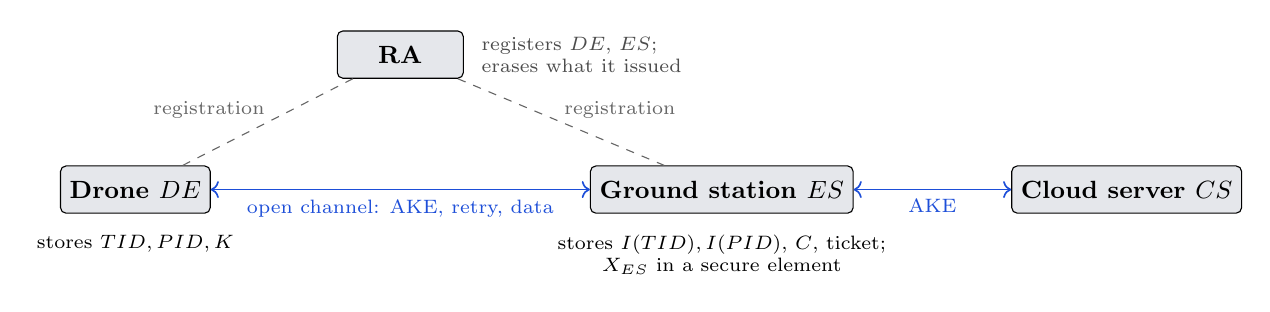
\begin{tikzpicture}[node distance=1.2cm and 2.2cm, font=\small]
  \node[party] (ra) {RA};
  \node[party, below left=1.1cm and 1.6cm of ra] (de) {Drone $DE$};
  \node[party, below right=1.1cm and 1.6cm of ra] (es) {Ground station $ES$};
  \node[party, right=2.0cm of es] (cs) {Cloud server $CS$};
  \draw[dashed, black!60] (ra) -- node[above left, font=\scriptsize, pos=0.5, fill=white, inner sep=1pt] {registration} (de);
  \draw[dashed, black!60] (ra) -- node[above right, font=\scriptsize, pos=0.5, fill=white, inner sep=1pt] {registration} (es);
  \draw[msg, <->] (de) -- node[below, font=\scriptsize] {open channel: AKE, retry, data} (es);
  \draw[msg, <->] (es) -- node[below, font=\scriptsize] {AKE} (cs);
  \node[font=\scriptsize, below=0.15cm of de, align=center] {stores $TID, PID, K$};
  \node[font=\scriptsize, below=0.15cm of es, align=center] {stores $I(TID), I(PID)$, $C$, ticket;\\ $X_{ES}$ in a secure element};
  \node[font=\scriptsize, right=0.1cm of ra, align=left, text=black!70] {registers $DE$, $ES$;\\ erases what it issued};
\end{tikzpicture}
\caption{Network model. Dashed lines: registration over a secure channel. Solid arrows: open channels controlled by the
attacker. The stored values are those of \cref{sec:scheme}.}
\label{fig:network}
\end{figure}

\begin{table*}[!t]
\centering
\footnotesize
\caption{Design rationale (\texttt{spec/changes.json}). Each change, the findings it addresses (F: BAKMM-IoD, \cref{tab:flaws}; O, R: findings on the predecessor v2 and of our specification review, listed in the artifact) and its cost effect.}
\label{tab:rationale}
\setlength{\tabcolsep}{3pt}
\begin{tabular}{p{6.4cm}p{1.6cm}p{6.6cm}}
\toprule
Change (BAKMM-IoD / v2 $\rightarrow$ v3) & Flaws & Cost effect \\
\midrule
Hash with domain-separation labels & F2, F3 & none (label bytes inside the same hash call) \\
Server erases K at commit; one record per drone & F4, O2 & none for the commit itself \\
Retry ticket & O2, F7 & server +1 hash (E9) and +1 AES (E10) per session; drone +1 hash and +1 AES only on a retry \\
Keyed one-time retry pseudonym & F7, O9 & none: same hash call as TID' \\
Next identity hashed with K & F5, F9, F10 & none \\
Encrypted database index and record; no XOR & F8, F9, O3 & server: 2 hashes of the XOR mask of v2 replaced by AES operations (5 senc + 1 sdec per session in total) \\
Key confirmation message & O4 & +1 hash each side, +256 bits \\
No timestamps & O6 & -32 bits per message \\
Data record with counter under AEAD & F11 & 1 AES operation per record (as BAKMM-IoD's encryption), +64-bit counter, +128-bit tag \\
Session keys never stored; all field lengths checked & O5 & none \\
Check values V2, V3 computed from K, not from SK & R8 & none (same number of hashes) \\
\bottomrule
\end{tabular}
\end{table*}


\subsection{Equations}
Every computation is written once; both sides of every check use the same numbered equation. The equations below are
generated from the specification.
{\small\setlength{\multlinegap}{0pt}% GENERATED from spec/fsl_ake_v3.md section 4 by paper/scripts/make_tables.py -- equations identical to the spec
\begin{multline*}\tag{E0}\label{eq:E0} X_{idx} = H(\text{``x-idx''}, X_{ES})[0..127]\;\text{,} \\ X_{db} = H(\text{``x-db''}, X_{ES})[0..127] \end{multline*}
\noindent{\footnotesize computed by: ES, once per boot}\par
\begin{multline*}\tag{E1}\label{eq:E1} I(id) = \mathrm{PRP}_{X_{idx}}(id) \\ \text{; being a permutation, ES reads}\;id\;\text{back as}\;\mathrm{PRP}^{-1}_{X_{idx}}(I(id)) \end{multline*}
\noindent{\footnotesize computed by: ES}\par
\begin{multline*}\tag{E2}\label{eq:E2} C = \mathrm{AEAD}_{X_{db}}(\nu ; K; \text{``rec''}  \|  dev)\;\text{,} \\ \nu \;\text{random, stored as}\;(\nu , C) \end{multline*}
\noindent{\footnotesize computed by: ES}\par
\begin{equation*}\tag{E3}\label{eq:E3} V_1 = H(\text{``v1''}, K, TID, N_1) \end{equation*}
\noindent{\footnotesize computed by: DE sends, ES checks}\par
\begin{equation*}\tag{E3r}\label{eq:E3r} V_{1r} = H(\text{``v1r''}, K, PID, N_{1r}) \end{equation*}
\noindent{\footnotesize computed by: DE sends, ES checks}\par
\begin{multline*}\tag{E4}\label{eq:E4} SK = H(\text{``sk''}, K, TID, n, N_2)\;\text{,} \\ n\;\text{=}\;N_1\;\text{(first attempt) or}\;N_{1r}\;\text{(retry)} \end{multline*}
\noindent{\footnotesize computed by: DE and ES}\par
\begin{equation*}\tag{E5}\label{eq:E5} V_2 = H(\text{``v2''}, K, TID, n, N_2) \end{equation*}
\noindent{\footnotesize computed by: ES sends, DE checks}\par
\begin{equation*}\tag{E6}\label{eq:E6} V_3 = H(\text{``v3''}, K, TID, n, N_2) \end{equation*}
\noindent{\footnotesize computed by: DE sends, ES checks}\par
\begin{equation*}\tag{E7}\label{eq:E7} K' = H(\text{``k''}, K, SK) \end{equation*}
\noindent{\footnotesize computed by: DE and ES}\par
\begin{multline*}\tag{E8}\label{eq:E8} W = H(\text{``id''}, K, TID, SK)\;\text{;} \\ TID' = W[0..159]\;\text{,} \\ PID' = W[160..255] \end{multline*}
\noindent{\footnotesize computed by: DE and ES}\par
\begin{equation*}\tag{E9}\label{eq:E9} R = H(\text{``r''}, K, TID, n)[0..127] \end{equation*}
\noindent{\footnotesize computed by: ES on every commit; DE only on a retry}\par
\begin{equation*}\tag{E10}\label{eq:E10} T = \mathrm{AEAD}_{R}(0^{96}; N_2; \text{``tkt''}) \end{equation*}
\noindent{\footnotesize computed by: ES; DE decrypts}\par
\begin{equation*}\tag{E11}\label{eq:E11} KD = SK[0..127] \end{equation*}
\noindent{\footnotesize computed by: DE and ES}\par
\begin{equation*}\tag{E12}\label{eq:E12} \text{data record}\;D = (ctr, \mathrm{AEAD}_{KD}(dir  \|  ctr; data; \text{``dat''}  \|  dir  \|  ctr)) \end{equation*}
\noindent{\footnotesize computed by: sender; receiver decrypts}\par
}

\subsection{Registration}
The RA picks $TID$, $PID$ and $K$ at random and a fresh device number $dev$, gives $(TID, PID, K)$ to the drone and
$(dev, TID, PID, K)$ to the ground station over a secure channel, and erases them (\cref{fig:registration}). The ground station
stores the indices $I(TID)$, $I(PID)$ (E1) and the record $(\nu, C)$ (E2).
\begin{figure*}[!t]
\centering
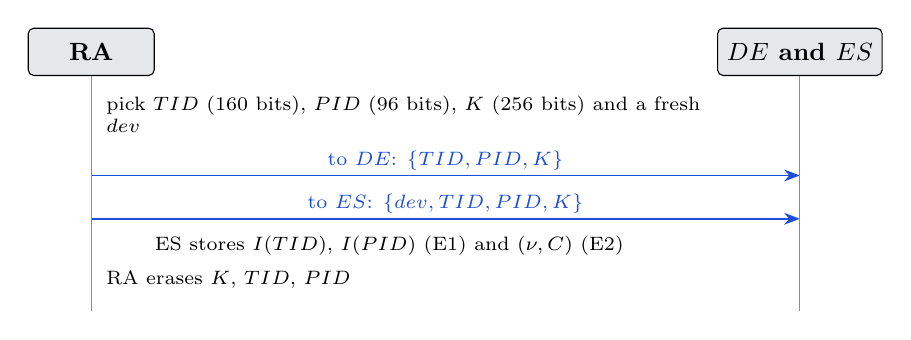
\begin{tikzpicture}
  \renewcommand{\msclen}{9.0}
  \mscstart{RA}{$DE$ and $ES$};
  \mscL[8.0cm]{pick $TID$ (160 bits), $PID$ (96 bits), $K$ (256 bits) and a fresh $dev$};
  \mscmsg{r}{to $DE$: $\{TID, PID, K\}$};
  \mscmsg{r}{to $ES$: $\{dev, TID, PID, K\}$};
  \mscR[8.0cm]{ES stores $I(TID)$, $I(PID)$ (E1) and $(\nu, C)$ (E2)};
  \mscL[8.0cm]{RA erases $K$, $TID$, $PID$};
  \mscend;
\end{tikzpicture}
\caption{Registration of FSL-AKE v3 (\texttt{spec/fsl\_ake\_v3.md}, \S6.1). Both arrows use the secure registration channel.}
\label{fig:registration}
\end{figure*}


\subsection{Drone--server authentication and key establishment}
\Cref{fig:ake} shows the three messages. The drone sends $MSG_1 = \{TID, N_1, V_1\}$. The ground station checks lengths, finds
the record by $I(TID)$, decrypts $K$ and checks $V_1$ (E3). It then picks $N_2$, computes $SK$ (E4), $V_2$ (E5), $V_3$ (E6),
$K'$ (E7), $TID'$ and $PID'$ (E8), $R$ (E9) and the ticket $T$ (E10), and commits atomically: it stores the new record over $K'$,
deletes the old record and the previous ticket, stores $T$ under the old index $I(PID)$, and erases $K$ and $R$. It sends
$MSG_2 = \{N_2, V_2\}$. The drone checks $V_2$ (E5), computes $SK$ (E4), and in one atomic step computes $V_3$, $K'$, $TID'$,
$PID'$, stores them and erases $K$, $TID$, $PID$ and $N_1$; it then sends $MSG_3 = \{V_3\}$. The ground station accepts $SK$
only if $V_3$ equals the pending value. The check values $V_2$ and $V_3$ are computed from $K$, so $SK$ enters no public value.
\begin{figure*}[!t]
\centering
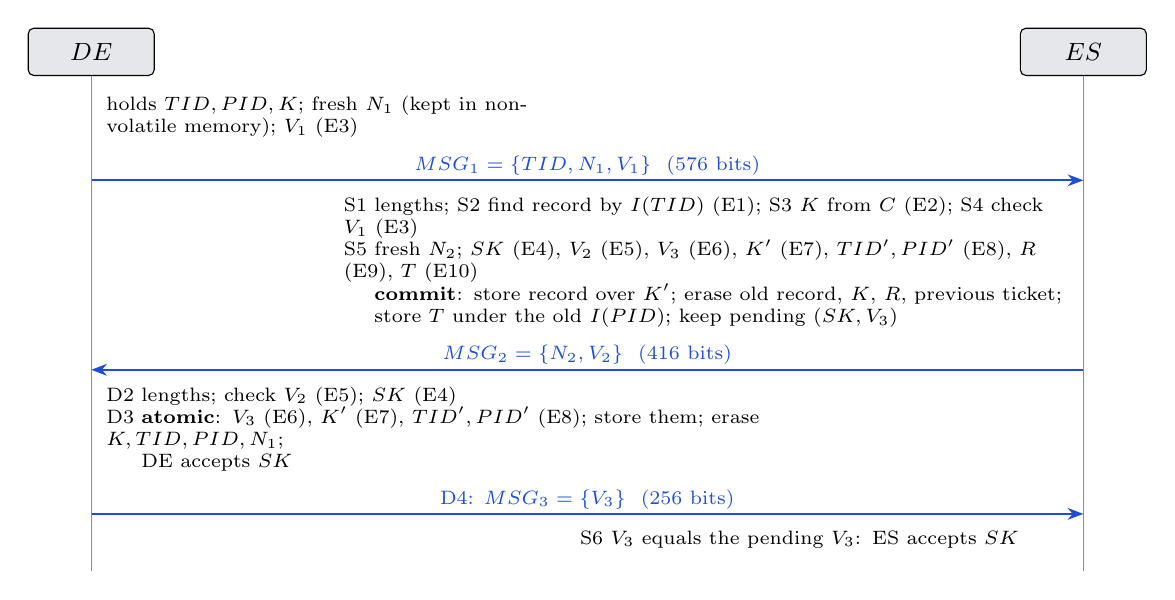
\begin{tikzpicture}
  \mscstart{$DE$}{$ES$};
  \mscL{holds $TID, PID, K$; fresh $N_1$ (kept in non-volatile memory); $V_1$ (E3)};
  \mscmsg{r}{$MSG_1=\{TID, N_1, V_1\}$ \ (576 bits)};
  \mscR[9.2cm]{S1 lengths; S2 find record by $I(TID)$ (E1); S3 $K$ from $C$ (E2); S4 check $V_1$ (E3)\\
        S5 fresh $N_2$; $SK$ (E4), $V_2$ (E5), $V_3$ (E6), $K'$ (E7), $TID', PID'$ (E8), $R$ (E9), $T$ (E10)\\
        \phantom{S5 }\textbf{commit}: store record over $K'$; erase old record, $K$, $R$, previous ticket;\\
        \phantom{S5 }store $T$ under the old $I(PID)$; keep pending $(SK, V_3)$};
  \mscmsg{l}{$MSG_2=\{N_2, V_2\}$ \ (416 bits)};
  \mscL[9.2cm]{D2 lengths; check $V_2$ (E5); $SK$ (E4)\\
        D3 \textbf{atomic}: $V_3$ (E6), $K'$ (E7), $TID', PID'$ (E8); store them; erase $K, TID, PID, N_1$;\\
        \phantom{D3 }DE accepts $SK$};
  \mscmsg{r}{D4: $MSG_3=\{V_3\}$ \ (256 bits)};
  \mscR{S6 $V_3$ equals the pending $V_3$: ES accepts $SK$};
  \mscend;
\end{tikzpicture}
\caption{Drone--server authentication and key establishment of FSL-AKE v3 (\texttt{spec/fsl\_ake\_v3.md}, \S6.2). S1--S6 are server steps, D2--D4 drone steps ($MSG_3$ is sent at D4); equation
numbers as in \cref{sec:scheme}. Party indices are dropped ($DE$, $ES$). No timestamps are used. Total \BitsVthree\ bits.}
\label{fig:ake}
\end{figure*}


\subsection{Retry}
If the drone gets no $MSG_2$ it sends $MSG_{1r} = \{PID, N_{1r}, V_{1r}\}$ (E3r). If $I(PID)$ still indexes the record,
$MSG_1$ was lost and the ground station runs the normal steps with $n = N_{1r}$; if it indexes a ticket, $MSG_2$ was lost and
the ground station returns $T$ unchanged, from which the drone recovers $N_2$ with $R$ (E9) (\cref{fig:retry}). The drone keeps
$N_1$ and $N_{1r}$ in non-volatile memory until it has an answer and never replaces them before D3; if it loses them it must be
registered again. A second retry resends the same $MSG_{1r}$, so at most one retry per session can be unlinkable, and only when
every candidate drone lost $MSG_2$ (Tamarin, fixed scenario); it is linkable if $MSG_2$ is dropped for one drone only
(\cref{sec:discussion}).
\begin{figure}[!htbp]
\centering
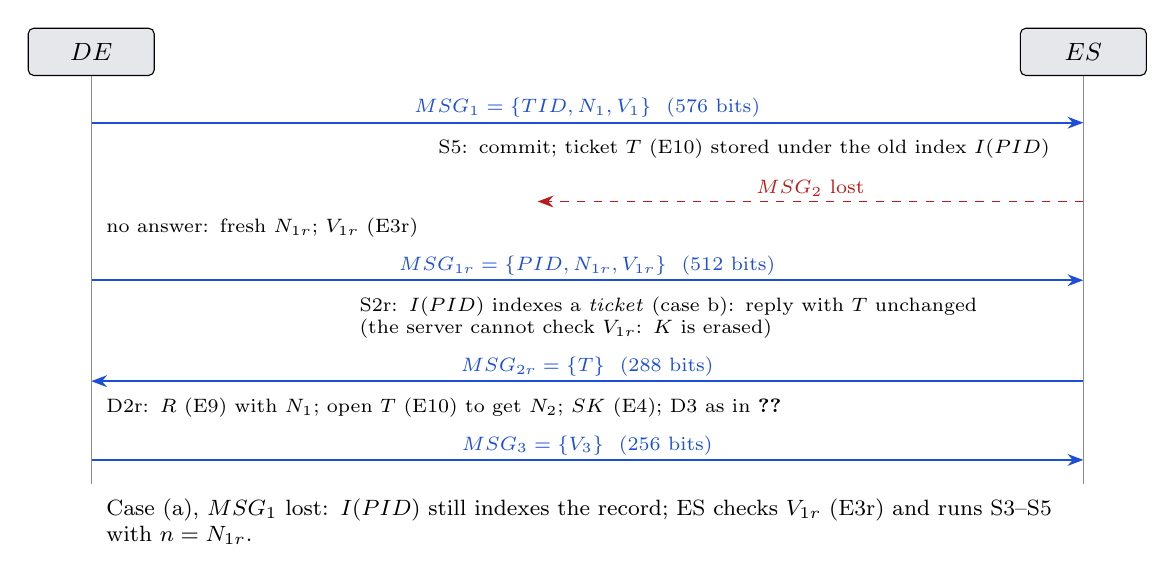
\begin{tikzpicture}
  \mscstart{$DE$}{$ES$};
  \mscmsg{r}{$MSG_1=\{TID, N_1, V_1\}$ \ (576 bits)};
  \mscR[8.0cm]{S5: commit; ticket $T$ (E10) stored under the old index $I(PID)$};
  \msclost{l}{$MSG_2$ lost};
  \mscL{no answer: fresh $N_{1r}$; $V_{1r}$ (E3r)};
  \mscmsg{r}{$MSG_{1r}=\{PID, N_{1r}, V_{1r}\}$ \ (512 bits)};
  \mscR[9.0cm]{S2r: $I(PID)$ indexes a \emph{ticket} (case b): reply with $T$ unchanged\\ (the server cannot check $V_{1r}$: $K$ is erased)};
  \mscmsg{l}{$MSG_{2r}=\{T\}$ \ (288 bits)};
  \mscL[9.0cm]{D2r: $R$ (E9) with $N_1$; open $T$ (E10) to get $N_2$; $SK$ (E4); D3 as in \cref{fig:ake}};
  \mscmsg{r}{$MSG_3=\{V_3\}$ \ (256 bits)};
  \mscend;
  \node[comp=12.3cm, anchor=north west, font=\footnotesize] at ($(prev)+(0.15,-0.4)$) {%
    Case (a), $MSG_1$ lost: $I(PID)$ still indexes the record; ES checks $V_{1r}$ (E3r) and runs S3--S5 with $n=N_{1r}$.};
\end{tikzpicture}
\caption{Retry path of FSL-AKE v3 (\texttt{spec/fsl\_ake\_v3.md}, \S6.3), case (b), $MSG_2$ lost: at most one retry per session can be unlinkable (only when every candidate drone lost $MSG_2$). The keyed pseudonym $PID$ comes from E8
of the previous session.}
\label{fig:retry}
\end{figure}


\subsection{Server--cloud phase, data records and revocation}
The server--cloud phase uses the same messages and equations with the ground station as initiator, holding $\{TIN, PIN, K\}$,
and the cloud server as responder. Data records carry a counter under AEAD (E11, E12, \cref{fig:record}); the receiver
accepts a record only if it decrypts and its counter is larger than the last accepted one. Revocation deletes the record, both
indices and the ticket of a device.
\begin{figure}[!htbp]
\centering
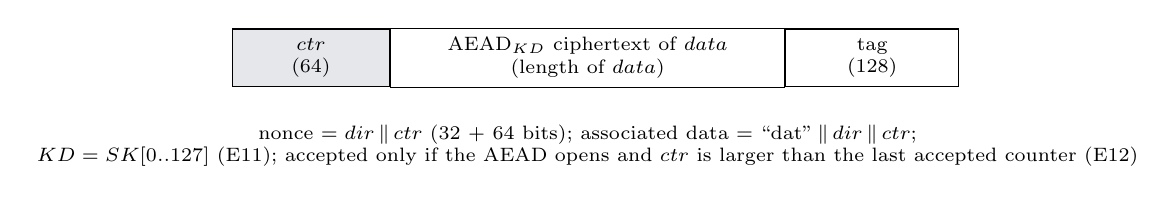
\begin{tikzpicture}[font=\scriptsize, cell/.style={draw, minimum height=0.7cm, align=center}]
  \node[cell, minimum width=2.0cm, fill=lightgrey] (c) at (0,0) {$ctr$\\(64)};
  \node[cell, minimum width=5.0cm, right=0pt of c] (ct) {$\mathrm{AEAD}_{KD}$ ciphertext of $data$\\(length of $data$)};
  \node[cell, minimum width=2.2cm, right=0pt of ct] (tag) {tag\\(128)};
  \node[font=\scriptsize, below=0.35cm of ct, align=center] {nonce $= dir\,\|\,ctr$ (32 + 64 bits); associated data $= \text{``dat''}\,\|\,dir\,\|\,ctr$;\\
     $KD = SK[0..127]$ (E11); accepted only if the AEAD opens and $ctr$ is larger than the last accepted counter (E12)};
\end{tikzpicture}
\caption{Data-record format of FSL-AKE v3 (\texttt{spec/fsl\_ake\_v3.md}, \S6.5): \num{192} bits plus the data.}
\label{fig:record}
\end{figure}


\section{Security analysis of FSL-AKE v3}\label{sec:security}

\subsection{Formal proof in the Real-Or-Random style (hand proof)}\label{sec:ror}
\emph{This subsection is a hand proof; it is not machine-checked.} It follows \texttt{spec/ror\_proof.md}, which went through
an internal review during the project (not an external peer review); objection R1 of that review led to the present form of
E5 and E6 (\cref{sec:scheme}).

\textbf{Assumptions.} (A1) each labelled hash is an independent random oracle with 256-bit output; (A2) AES-128-GCM is a
multi-query secure AEAD (IND-CPA and INT-CTXT) with advantage $\mathrm{Adv}^{ae}$ per key; (A3) the index E1 depends only on
the identifier and $X_{idx}$; (A4) erased values are not available to later corruptions; (A5) registration runs over a secure
channel and the RA erases what it issued; (A6) nonces, the first $K$ and $X_{ES}$ are uniform.

\textbf{Queries and freshness.} The adversary uses \textsf{Execute}, \textsf{Send}, \textsf{Reveal} (a session key),
\textsf{CorruptDE} (the drone's memory), \textsf{CorruptDB} (the server database), \textsf{CorruptState} (the server's
pending and running keys), \textsf{CorruptX} ($X_{ES}$), \textsf{RevealEph} and one \textsf{Test}. A drone instance and a
server instance \emph{match} if they used the same $(TID, n, N_2)$. An accepted instance is fresh if (1) no \textsf{Reveal}
of it or of a matching instance; (2) no \textsf{CorruptDE} before its drone erased $SK$; (3) no \textsf{CorruptState} before the
matching server instance erased $SK$, and no \textsf{CorruptDB} together with \textsf{CorruptX} before the record holding this
session's $K$ was erased. Condition (2) excludes F6, condition (3) excludes F8 with $X_{ES}$, and the absence of corruption
before a session excludes post-compromise security.

\textbf{Theorem.} With $q = q_s + q_e$ \textsf{Send} and \textsf{Execute} queries and $q_h$ oracle queries,
\begin{multline*}
\mathrm{Adv} \le \frac{q_h^2}{2^{256}} + \frac{9q^2}{2^{160}} + \frac{q^2}{2^{96}} + \frac{q_s}{2^{255}} \\ + \frac{q_h}{2^{126}}
 + \frac{q_h(q+1)}{2^{255}} + 4(q+1)\,\mathrm{Adv}^{ae}.
\end{multline*}

\textbf{Game sequence.} \\
G0 is the real attack. \\
G1 simulates the random oracles by tables (no change). \\
G2 aborts on collisions of oracle outputs, of the up to three nonces per session, and of the 96-bit pseudonyms (the last affects only availability). \\
G3 aborts if the adversary queries an oracle input containing the key $K$ of a fresh session, or $X_{ES}$ without corrupting
it; by induction over the key chain each $K$ is uniform to the adversary until it is erased. \\
G4 replaces every stored record $C$ and ticket $T$ by encryptions of zeros (A2). \\
G5 aborts on accepted check values or tickets the partner did not produce; after G5 every accepting server has a matching accepting drone (key confirmation). \\
In G6 the tested $SK = H(\text{``sk''}, K, TID, n, N_2)$ has an unqueried input used by no other session, and no public value is a function of
$SK$, so the Test answer is independent of the adversary's view. \\ 
Doubling the sum of the differences gives the bound: G2
gives the first three terms (oracle-output, nonce and pseudonym collisions), G3 the terms $q_h(q+1)/2^{255}$ (guessing a
chain key) and $q_h/2^{126}$ (guessing the 128-bit $X_{ES}$ in either of its two oracle inputs), G5 the term $q_s/2^{255}$
(forging a check value), and G4 and G5 one $(q+1)\mathrm{Adv}^{ae}$ each (hiding and forging records and tickets).

\subsection{Automated verification with Tamarin}\label{sec:tamarin}
\textbf{Modelling.} The protocol state is held in linear facts that are consumed when the protocol moves on (explicit
erasure); each stored value also has a persistent memory copy that only reveal rules read, and a restriction forbids reading a
value after it was erased. The reveal rules are those of the threat model (\cref{sec:threat}). The same lemma text and reveal
rules are applied to the v2 predecessor and to a BAKMM-IoD model, so that results can be compared lemma by lemma.

\textbf{Bounds.} The unbounded drone--server model was killed for lack of memory on its executability lemma. All drone--server
results are therefore \emph{bounded}: one consecutive session per drone--server pair; the three lemmas that need two sessions
use a two-session bound. The data-path theory is unbounded; the unlinkability theories are a fixed scenario of two drones and
one retry. Every v3 drone--server, server--cloud, data-path and unlinkability theory has a verified executability lemma
(\cref{tab:tamarin,tab:tamarin-extra}); the two-session executability of the BAKMM-IoD model did not terminate.

\textbf{Results.} \Cref{tab:tamarin} gives the drone--server lemmas. On v3, \NumVthreeVerified\ of \NumVthreeLemmas\ lemmas
are verified; the \NumVthreeFalsified\ falsified ones are the stated limits (post-compromise security, F6, F8 with $X_{ES}$),
each with a trace we read. Of the \NumBakmmBaseLemmas\ BAKMM-IoD lemmas under the same text, \NumBakmmBaseDNT\ did not
terminate within the 7.7\,GB memory limit, also after two changes of the prover settings; only its one-session
executability terminated. The server--cloud theory verifies \NumCSverified\ of \NumCSlemmas\ lemmas (one session per pair). \Cref{tab:tamarin-extra} gives the
data path, where BAKMM-IoD's \texttt{no\_replay\_data} is falsified and v3's verified, and unlinkability, where v3 is verified
when every candidate drone lost $MSG_2$ and falsified when $MSG_2$ is dropped for exactly one drone.
Every verdict in \cref{tab:tamarin,tab:tamarin-extra} is read from a saved prover output, one file per lemma, in
\texttt{results/tamarin/main/<theory>/<lemma>.txt} (line~2 holds the verdict, step count and time).
\begin{table*}[!t]
\centering
\footnotesize
\caption{Tamarin results, drone--server phase. Same lemma text and reveal rules for all three models; \emph{Sess.}: bound, consecutive sessions per drone--server pair. DNT: did not terminate (killed for lack of memory, 7.7\,GB). Limit lemmas are expected to be falsified. $^\dagger$Backward secrecy: knowledge of a session key does not reveal any earlier session key.}
\label{tab:tamarin}
\setlength{\tabcolsep}{3pt}
\begin{tabular}{p{3.9cm}p{4.0cm}cccccc}
\toprule
Lemma & Property & BAKMM-IoD & v2 & v3 & Sess. & Steps & Time (s) \\
\midrule
\texttt{executable} & honest session runs (executability) & verified & verified & \textbf{verified} & 1 & 12 & 15 \\
\texttt{executable\_\allowbreak{}retry\_\allowbreak{}lost\_\allowbreak{}msg2} & retry after lost MSG2 runs & n/a & n/a & \textbf{verified} & 1 & 13 & 10 \\
\texttt{executable\_\allowbreak{}retry\_\allowbreak{}lost\_\allowbreak{}msg1} & retry after lost MSG1 runs & n/a & n/a & \textbf{verified} & 1 & 15 & 8 \\
\texttt{secrecy\_\allowbreak{}SK} & session-key secrecy (drone view) & DNT & verified & \textbf{verified} & 1 & 155 & 17 \\
\texttt{secrecy\_\allowbreak{}SK\_\allowbreak{}server} & session-key secrecy (server view) & DNT & verified & \textbf{verified} & 1 & 75 & 12 \\
\texttt{inj\_\allowbreak{}agree\_\allowbreak{}drone} & injective agreement, drone & DNT & verified & \textbf{verified} & 1 & 132 & 9 \\
\texttt{inj\_\allowbreak{}agree\_\allowbreak{}server} & injective agreement, server & DNT & verified & \textbf{verified} & 1 & 54 & 8 \\
\texttt{key\_\allowbreak{}confirmation\_\allowbreak{}server} & key confirmation to the server & DNT & falsified & \textbf{verified} & 1 & 35 & 9 \\
\texttt{forward\_\allowbreak{}secrecy\_\allowbreak{}drone} & forward secrecy, drone side & DNT & verified & \textbf{verified} & 1 & 133 & 12 \\
\texttt{forward\_\allowbreak{}secrecy\_\allowbreak{}server} & forward secrecy, server side & DNT & falsified & \textbf{verified} & 1 & 66 & 9 \\
\texttt{forward\_\allowbreak{}secrecy\_\allowbreak{}all} & forward secrecy, both sides & DNT & falsified & \textbf{verified} & 1 & 133 & 11 \\
\texttt{other\_\allowbreak{}session\_\allowbreak{}key\_\allowbreak{}leak} & known session key & DNT & verified & \textbf{verified} & 1 & 155 & 16 \\
\texttt{ephemeral\_\allowbreak{}leak} & ephemeral leak (KSSTI/ESL) & DNT & verified & \textbf{verified} & 1 & 292 & 26 \\
\texttt{tid\_\allowbreak{}agreement} & next identity agreed & DNT & verified & \textbf{verified} & 1 & 48 & 9 \\
\texttt{tid\_\allowbreak{}secrecy} & next identity secret & DNT & falsified & \textbf{verified} & 1 & 142 & 17 \\
\texttt{no\_\allowbreak{}replay\_\allowbreak{}m1} & no replay of MSG1/MSG1r & DNT & verified & \textbf{verified} & 1 & 28 & 6 \\
\texttt{executable\_\allowbreak{}two\_\allowbreak{}sessions} & two sessions run (executability) & DNT & verified & \textbf{verified} & 2 & 20 & 670 \\
\texttt{backward\_\allowbreak{}secrecy\_\allowbreak{}paper\_\allowbreak{}def} & backward secrecy$^\dagger$ & DNT & verified & \textbf{verified} & 2 & 1137 & 154 \\
\texttt{pcs\_\allowbreak{}after\_\allowbreak{}K\_\allowbreak{}leak} & post-compromise security (limit O1) & DNT & falsified & \textbf{falsified} & 2 & 16 & 622 \\
\texttt{captured\_\allowbreak{}drone\_\allowbreak{}accepts\_\allowbreak{}false\_\allowbreak{}server} & captured drone rejects false server (limit F6) & DNT & falsified & \textbf{falsified} & 1 & 8 & 8 \\
\texttt{drone\_\allowbreak{}impersonation\_\allowbreak{}with\_\allowbreak{}db\_\allowbreak{}and\_\allowbreak{}X} & database + $X_{ES}$ cannot impersonate (limit F8) & DNT & falsified & \textbf{falsified} & 1 & 10 & 9 \\
\bottomrule
\end{tabular}
\end{table*}

\begin{table*}[!t]
\centering
\footnotesize
\caption{Tamarin results for the data path (theories \texttt{*\_data\_only}, unbounded) and for unlinkability of a retry (observational equivalence, fixed scenario of two drones and one retry).}
\label{tab:tamarin-extra}
\setlength{\tabcolsep}{3pt}
\begin{tabular}{p{3.9cm}p{4.0cm}cccccc}
\toprule
Lemma & Property & BAKMM-IoD & v2 & v3 & Bound & Steps & Time (s) \\
\midrule
\texttt{executable\_\allowbreak{}data} & data path runs & verified & - & \textbf{verified} & unbounded & 8 & 0 \\
\texttt{no\_\allowbreak{}replay\_\allowbreak{}data} & data record accepted once (F11) & falsified & - & \textbf{verified} & unbounded & 2 & 0 \\
\texttt{data\_\allowbreak{}integrity} & data integrity & verified & - & \textbf{verified} & unbounded & 6 & 0 \\
\texttt{data\_\allowbreak{}secrecy} & data secrecy & verified & - & \textbf{verified} & unbounded & 5 & 0 \\
\texttt{Observational\_\allowbreak{}equivalence} & retry unlinkable, both drones lost MSG2 (F7) & falsified & falsified & \textbf{verified} & scenario & 443 & 13 \\
\texttt{Observational\_\allowbreak{}equivalence} & retry unlinkable, MSG2 dropped for one drone (limit) & - & - & \textbf{falsified} & scenario & 8 & 9 \\
\bottomrule
\end{tabular}
\end{table*}


\subsection{Automated verification with Scyther}\label{sec:scyther}
We model v3 in the style of the BAKMM-IoD listing, one protocol branch per file, and give the BAKMM-IoD listing (made
runnable) exactly the same claim set. Both are verified with the same settings. \Cref{tab:scyther} compares them. For v3 every
explicit claim of the normal path is a proof of correctness. For BAKMM-IoD at the bound that finishes (3 runs; 5 runs did not finish
within \ScyBakmmFiveSecs\,s), \texttt{Niagree} and \texttt{Nisynch} fail for both roles: the attack trace alters $M_5$ (F5). In
the retry branch of v3, \texttt{Niagree} and \texttt{Nisynch} fail by design, because the ground station cannot check
$MSG_{1r}$ after erasing $K$; agreement on $SK$ (\texttt{Commit}) holds. Scyther cannot express forward or backward secrecy,
key evolution or unlinkability; those are shown with Tamarin only.
\begin{table}[!htbp]
\centering
\footnotesize
\caption{Scyther v1.3.0, identical claim set for both protocols. \emph{Ok (proof)}: proof of correctness, valid for any number of runs; \emph{Ok (bound)}: no attack within the bound. BAKMM-IoD at 5 runs did not finish within 600\,s.}
\label{tab:scyther}
\setlength{\tabcolsep}{3pt}
\begin{tabular}{llllll}
\toprule
Role & Claim & BAKMM-IoD, 3 runs & v3, 3 runs & v3, 5 runs & v3, 9 runs \\
\midrule
DE & Secret long-term key & Ok (bound) & Ok (proof) & Ok (proof) & Ok (proof) \\
DE & Secret SK & Ok (bound) & Ok (proof) & Ok (proof) & Ok (proof) \\
DE & SKR(SK) & Ok (bound) & Ok (proof) & Ok (proof) & Ok (proof) \\
DE & Alive & Ok (bound) & Ok (proof) & Ok (proof) & Ok (proof) \\
DE & Weakagree & Ok (bound) & Ok (proof) & Ok (proof) & Ok (proof) \\
DE & Niagree & Fail & Ok (proof) & Ok (proof) & Ok (proof) \\
DE & Nisynch & Fail & Ok (proof) & Ok (proof) & Ok (proof) \\
DE & Commit(SK) & Ok (bound) & Ok (proof) & Ok (proof) & Ok (proof) \\
ES & Secret long-term key & Ok (bound) & Ok (proof) & Ok (proof) & Ok (proof) \\
ES & Secret SK & Ok (bound) & Ok (proof) & Ok (proof) & Ok (proof) \\
ES & SKR(SK) & Ok (bound) & Ok (proof) & Ok (proof) & Ok (proof) \\
ES & Alive & Ok (bound) & Ok (proof) & Ok (proof) & Ok (proof) \\
ES & Weakagree & Ok (bound) & Ok (proof) & Ok (proof) & Ok (proof) \\
ES & Niagree & Fail & Ok (proof) & Ok (proof) & Ok (proof) \\
ES & Nisynch & Fail & Ok (proof) & Ok (proof) & Ok (proof) \\
ES & Commit(SK) & Ok (bound) & Ok (proof) & Ok (proof) & Ok (proof) \\
\bottomrule
\end{tabular}
\end{table}


\textbf{Explicit versus auto-generated claims.} The nonces $N_1$, $N_{1r}$ and $N_2$ are public freshness values: they are
sent in clear in $MSG_1$, $MSG_{1r}$ and $MSG_2$, and no equation relies on their secrecy, since $SK$ (E4), $V_1$ (E3), $V_2$ (E5)
and $V_3$ (E6) all take the key $K$ as input. Our verification therefore checks only the explicit claims of
\cref{tab:scyther}. Scyther's \emph{Autoverify} (\texttt{--auto-claims}) replaces them by generated claims, including
\texttt{Secret} for every fresh value; on the normal path it reports \ScyAutoNormalAutoOk\ claims Ok and
\ScyAutoNormalAutoFail\ Fail, on the retry branch \ScyAutoRetryAutoOk\ Ok and \ScyAutoRetryAutoFail\ Fail
(\cref{tab:scyther-auto}). Each failing \texttt{Secret} claim concerns a nonce or the field $V_{1r}$, which the protocol sends
in clear, and its attack graph is an honest run in which the attacker only reads the messages; in the same models the explicit
\texttt{Secret} and \texttt{SKR} claims on $SK$ hold although the attacker knows every nonce. The failing \texttt{Niagree} and
\texttt{Nisynch} claims of the retry branch are the by-design failures discussed above. Tamarin's \texttt{ephemeral\_leak}
lemma, in which the nonces are revealed, is verified (\cref{tab:tamarin}). Results were identical at 3, 4 and 5 runs.
Panel (h) of \cref{fig:shots-scyther2} shows the Autoverify window of the normal path with its four failing \texttt{Secret}
claims.
\begin{table*}[!t]
\centering
\footnotesize
\caption{Scyther's auto-generated claims (GUI \emph{Autoverify}, CLI \texttt{--auto-claims}) on the v3 models, 5 runs; identical at 3 and 4 runs. They replace the explicit claims of \cref{tab:scyther}; the normal-path window is panel (h) of \cref{fig:shots-scyther2}. Every failing \texttt{Secret} claim concerns a value that the protocol sends in clear; the attack graphs (\texttt{results/scyther/autoclaims/}) are honest runs observed by a passive attacker. \texttt{V1rx} is the name, in \texttt{scyther/fsl\_v3\_de\_es\_retry.spdl}, of the server's variable that receives the field $V_{1r}$ of $MSG_{1r}$.}
\label{tab:scyther-auto}
\setlength{\tabcolsep}{3pt}
\begin{tabular}{llp{2.6cm}lp{2.6cm}p{5.6cm}}
\toprule
Branch & Role & Auto-claim & Verdict & Scyther note & Explanation \\
\midrule
normal & DE & Secret N1 & Fail & at least 1 attack & public by design: in clear in $MSG_1$; honest run, passive attacker \\
normal & DE & Secret N2 & Fail & at least 1 attack & public by design: in clear in $MSG_2$; honest run, passive attacker \\
normal & DE & Alive & Ok & proof of correctness &  \\
normal & DE & Weakagree & Ok & proof of correctness &  \\
normal & DE & Niagree & Ok & proof of correctness &  \\
normal & DE & Nisynch & Ok & proof of correctness &  \\
normal & ES & Secret N2 & Fail & at least 1 attack & public by design: in clear in $MSG_2$; honest run, passive attacker \\
normal & ES & Secret N1 & Fail & at least 1 attack & public by design: in clear in $MSG_1$; honest run, passive attacker \\
normal & ES & Alive & Ok & proof of correctness &  \\
normal & ES & Weakagree & Ok & proof of correctness &  \\
normal & ES & Niagree & Ok & proof of correctness &  \\
normal & ES & Nisynch & Ok & proof of correctness &  \\
retry & DE & Secret N1r & Fail & at least 1 attack & public by design: in clear in $MSG_{1r}$; honest run, passive attacker \\
retry & DE & Secret N1 & Fail & at least 1 attack & public by design: in clear in $MSG_1$; honest run, passive attacker \\
retry & DE & Secret N2 & Fail & at least 1 attack & public by design: in clear in $MSG_2$; honest run, passive attacker \\
retry & DE & Alive & Ok & proof of correctness &  \\
retry & DE & Weakagree & Ok & proof of correctness &  \\
retry & DE & Niagree & Fail & at least 1 attack & by design: server cannot check $MSG_{1r}$ after erasing $K$ \\
retry & DE & Nisynch & Fail & at least 1 attack & by design: server cannot check $MSG_{1r}$ after erasing $K$ \\
retry & ES & Secret N2 & Fail & at least 1 attack & public by design: in clear in $MSG_2$; honest run, passive attacker \\
retry & ES & Secret V1rx & Fail & at least 1 attack & public by design: the $V_{1r}$ field, in clear in $MSG_{1r}$; honest run, passive attacker \\
retry & ES & Secret N1r & Fail & at least 1 attack & public by design: in clear in $MSG_{1r}$; honest run, passive attacker \\
retry & ES & Secret N1 & Fail & at least 1 attack & public by design: in clear in $MSG_1$; honest run, passive attacker \\
retry & ES & Alive & Ok & no attack within bounds &  \\
retry & ES & Weakagree & Ok & no attack within bounds &  \\
retry & ES & Niagree & Fail & at least 1 attack & by design: server cannot check $MSG_{1r}$ after erasing $K$ \\
retry & ES & Nisynch & Fail & at least 1 attack & by design: server cannot check $MSG_{1r}$ after erasing $K$ \\
\bottomrule
\end{tabular}
\end{table*}


\textbf{Result windows.} \Cref{fig:shots-scyther} shows the Scyther windows for the comparison: BAKMM-IoD with v3's claim set,
where only \texttt{Niagree} and \texttt{Nisynch} fail (F5, panel a), v3 with the same claims (panel b), and role
characterisation, where both roles of both models are reachable (panels c, d). \Cref{fig:shots-scyther2} shows the retry branch
with its by-design failures (panel e), the server--cloud phase with every claim verified (panel f), the published BAKMM-IoD
listing, in which no role is reachable (panel g, F1), and the Autoverify window discussed above (panel h). Every verdict
visible in these windows equals the corresponding entry of \cref{tab:scyther,tab:scyther-auto} and of
\texttt{results/scyther/summary.json}.

\begin{figure*}[!t]
\centering
\shot{bakmm_verify}{(a) BAKMM-IoD, same claims as v3, Verify claims, 3 runs (12 Ok, 4 Fail).}{fig:shot-a6}\hfill
\shot{fsl_v3_de_es_verify}{(b) FSL-AKE v3, Verify claims, 5 runs (16 Ok, proof of correctness).}{fig:shot-a2}\\[4pt]
\shot{bakmm_same_claims_characterize}{(c) BAKMM-IoD, Characterize roles, 5 runs: both roles reachable, at least 10 trace patterns.}{fig:shot-a5}\hfill
\shot{fsl_v3_de_es_characterize}{(d) FSL-AKE v3, Characterize roles, 5 runs: both roles reachable, exactly 1 trace pattern each.}{fig:shot-a1}
\caption{Scyther result windows, normal path (scyther-gui, File $>$ Open, maximum number of runs as stated, other settings
default). BAKMM-IoD is verified at 3 runs because its 5-run verification did not finish within \ScyBakmmFiveSecs\,s.}
\label{fig:shots-scyther}
\end{figure*}

\begin{figure*}[!t]
\centering
\shot{fsl_v3_de_es_retry_verify}{(e) FSL-AKE v3 retry branch, Verify claims, 5 runs: \texttt{Niagree}, \texttt{Nisynch} fail by design (12 Ok, 4 Fail).}{fig:shot-a3}\hfill
\shot{fsl_v3_es_cs_verify}{(f) FSL-AKE v3 server--cloud phase, Verify claims, 5 runs (16 Ok, proof of correctness).}{fig:shot-a4}\\[4pt]
\shot{bakmm_paper_listing_characterize}{(g) The BAKMM-IoD paper's own listing, Characterize roles, 5 runs: no role reachable (F1).}{fig:shot-a7}\hfill
\shot{fsl_v3_de_es_autoverify}{(h) FSL-AKE v3, Autoverify (auto-generated claims): \texttt{Secret} $N_1$, $N_2$ fail because both
are sent in clear; agreement claims Ok (8 Ok, 4 Fail, \cref{tab:scyther-auto}).}{fig:shot-auto}
\caption{Scyther result windows, retry branch, server--cloud phase, published listing and auto-generated claims (settings as in
\cref{fig:shots-scyther}).}
\label{fig:shots-scyther2}
\end{figure*}

\subsection{Informal analysis}\label{sec:informal}
Each paragraph names the Tamarin lemma that backs it and its bound (\cref{tab:tamarin,tab:tamarin-extra}); the arguments
themselves are informal.
\textbf{Mutual authentication and key confirmation.} The drone accepts only a $V_2$ (E5) and the server only a $V_1$ (E3) or
$V_{1r}$ (E3r), all of which need $K$; the server accepts $SK$ only with $V_3$ (E6). Backed by \texttt{inj\_agree\_drone},
\texttt{inj\_agree\_server} and \texttt{key\_confirmation\_server} (one session per pair).
\textbf{Session-key secrecy and known session key.} $SK$ (E4) needs $K$, which is never sent; each session has its own $K$.
Backed by \texttt{secrecy\_SK} and \texttt{other\_session\_key\_leak} (one session per pair).
\textbf{Forward secrecy} (compromise of any party's long-term or current state does not reveal session keys of sessions that
completed before the compromise). $K$ and its record are erased at S5 and D3, $K' = H(\text{``k''}, K, SK)$ (E7) is one-way, and
the ticket needs $R$ (E9) from the erased $K$ (\cref{fig:timeline}). Backed by \texttt{forward\_secrecy\_drone},
\texttt{\_server} and \texttt{\_all} (one session per pair).
\begin{figure*}[!t]
\centering
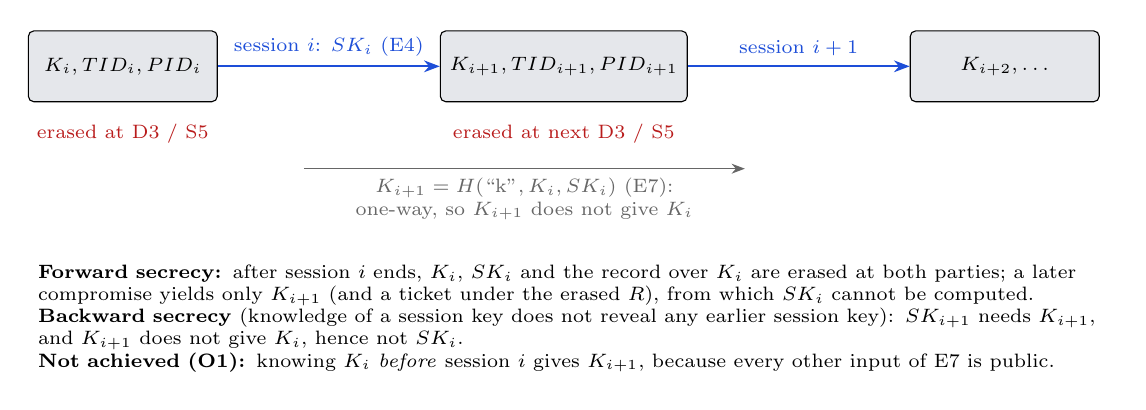
\begin{tikzpicture}[font=\scriptsize, st/.style={draw, rounded corners=2pt, align=center, minimum width=2.4cm, minimum height=0.9cm, fill=lightgrey}]
  \node[st] (s0) at (0,0) {$K_i, TID_i, PID_i$};
  \node[st] (s1) at (5.6,0) {$K_{i+1}, TID_{i+1}, PID_{i+1}$};
  \node[st] (s2) at (11.2,0) {$K_{i+2}, \dots$};
  \draw[msg] (s0) -- node[above, font=\scriptsize] {session $i$: $SK_i$ (E4)} (s1);
  \draw[msg] (s1) -- node[above, font=\scriptsize] {session $i+1$} (s2);
  \node[font=\scriptsize, below=0.15cm of s0, text=warn] {erased at D3 / S5};
  \node[font=\scriptsize, below=0.15cm of s1, text=warn] {erased at next D3 / S5};
  \draw[-{Stealth}, black!60] (2.3,-1.3) -- node[below, font=\scriptsize, align=center] {$K_{i+1} = H(\text{``k''}, K_i, SK_i)$ (E7):\\ one-way, so $K_{i+1}$ does not give $K_i$} (7.9,-1.3);
  \node[font=\scriptsize, align=left, text width=13.6cm, anchor=north west] at (-1.2,-2.4) {%
    \textbf{Forward secrecy:} after session $i$ ends, $K_i$, $SK_i$ and the record over $K_i$ are erased at both parties; a
    later compromise yields only $K_{i+1}$ (and a ticket under the erased $R$), from which $SK_i$ cannot be computed.\\
    \textbf{Backward secrecy} (knowledge of a session key does not reveal any earlier session key): $SK_{i+1}$ needs $K_{i+1}$,
    and $K_{i+1}$ does not give $K_i$, hence not $SK_i$.\\
    \textbf{Not achieved (O1):} knowing $K_i$ \emph{before} session $i$ gives $K_{i+1}$, because every other input of E7 is public.};
\end{tikzpicture}
\caption{Key evolution and erasure in FSL-AKE v3 and why forward and backward secrecy hold (Tamarin, bounded; the argument in the figure is informal; \cref{sec:security}).}
\label{fig:timeline}
\end{figure*}

\textbf{Backward secrecy} (knowledge of a session key does not reveal any earlier session key). $SK_{i+1}$ needs $K_{i+1}$,
which does not give $K_i$. Backed by \texttt{backward\_secrecy\_paper\_def}, two sessions per pair.
\textbf{Ephemeral leak.} The nonces are public by design; $SK$ also needs $K$. Backed by \texttt{ephemeral\_leak} (one session
per pair). Ephemeral values together with $K$ do give $SK$ (no Diffie--Hellman step).
\textbf{Identity.} $TID'$ and $PID'$ come from E8, which includes $K$; the database holds them only as indices (E1). Backed by
\texttt{tid\_agreement} and \texttt{tid\_secrecy} (one session per pair; the database may be read, but not together with
$X_{ES}$).
\textbf{Replay.} The record of $(TID, K)$ is deleted at commit, so a replayed $MSG_1$ finds no record; data records need a
larger counter (E12). Backed by \texttt{no\_replay\_m1} (one session per pair) and \texttt{no\_replay\_data} (data-path theory,
unbounded).
\textbf{Untraceability.} A retry uses the keyed one-time $PID$; it is unlinkable when every candidate drone lost $MSG_2$, but
not when the attacker drops $MSG_2$ for exactly one drone (\cref{sec:discussion}). Backed by observational equivalence in the
fixed scenario of two drones and one retry (\texttt{fsl\_v3\_unlink} verified, \texttt{fsl\_v3\_unlink\_mixed} falsified).
\textbf{No clock synchronisation.} No timestamps are used (a design property; no lemma).

\subsection{Security comparison}\label{sec:comparison}
\Cref{tab:checklist} compares BAKMM-IoD and v3 over the 38 checklist items under one rule: \emph{better} only if the BAKMM-IoD
result is falsified and the v3 result verified for the same lemma text, attacker and bound, or, where the BAKMM-IoD Tamarin model
did not terminate, for the identical Scyther claim set at 3 runs; a row with several lemmas takes the weakest of their
comparisons. The only BAKMM-IoD verdict available for many items is the Scyther \texttt{Niagree}/\texttt{Nisynch} failure, and
every attack graph of that failure is the F5 alteration of $M_5$; it does not show a man-in-the-middle, impersonation,
parallel-session or verifier-table attack, and \texttt{Commit} on $SK$ holds. The \DomFiveOnly\ items that name such an attack,
or session-key agreement or freshness (items 2, 3, 14--17, 28), are therefore not comparable; item~1 (mutual authentication) is
equal because its key-confirmation lemma is equal. Under this rule v3 is better on \DomBetter\ item (untraceability, item~33),
equal on \DomEqual, worse on \DomWorse, and not comparable on \DomNC. Most not-comparable rows have no BAKMM-IoD verdict because
its Tamarin model did not terminate, or concern properties without a lemma; they are kept visible with the reason. Over the
BAKMM-IoD rows including the findings F1--F11 (\cref{tab:flawrows}, Tamarin only) the counts are \DomAllBetter\ better,
\DomAllEqual\ equal, \DomAllWorse\ worse and \DomAllNC\ not comparable. The rows O1--O7 compare the predecessor v2 with v3
(\DomVtwoBetter\ better, \DomVtwoEqual\ equal, \DomVtwoWorse\ worse, \DomVtwoNC\ not comparable) and are not part of these counts.
\begin{table*}[!t]
\centering
\footnotesize
\caption{Security comparison over the 38 checklist items. A row is \emph{better} only if the BAKMM-IoD result is falsified and the v3 result verified under the same lemma text, reveal rules and bound, or, where the BAKMM-IoD Tamarin model did not terminate, for the identical Scyther claim set at 3 runs (Scy); \emph{equal} if both agree (shared limits included); \emph{not comparable} otherwise, e.g.\ when the BAKMM-IoD model did not terminate (DNT). A row with several lemmas takes the weakest of their comparisons. In every (Scy) row the BAKMM-IoD failure is the F5 alteration of $M_5$ (all 60 attack graphs at 3 runs, in \texttt{results/scyther/attacks/}); rows whose item names another attack (2, 3, 14--17, 28) are therefore not comparable, the reason being in \texttt{results/dominance.md}.}
\label{tab:checklist}
\setlength{\tabcolsep}{2.5pt}
\begin{tabular}{rp{3.0cm}p{4.3cm}p{2.5cm}p{2.0cm}l}
\toprule
\# & Item & Lemma(s) & BAKMM-IoD & v3 & Comparison \\
\midrule
1 & Mutual authentication & \texttt{inj\_\allowbreak{}agree\_\allowbreak{}drone}, \texttt{inj\_\allowbreak{}agree\_\allowbreak{}server}, \texttt{key\_\allowbreak{}confirmation\_\allowbreak{}server} & attack (Scy, 3 runs); attack (Scy, 3 runs); no attack within 3 runs (Scy) & proof of correctness (Scy); proof of correctness (Scy); proof of correctness (Scy) & \textbf{equal} \\
2 & Session key agreement & \texttt{inj\_\allowbreak{}agree\_\allowbreak{}drone} & attack (Scy, 3 runs) & proof of correctness (Scy) & \textbf{not comparable} \\
3 & Key freshness & \texttt{inj\_\allowbreak{}agree\_\allowbreak{}drone} & attack (Scy, 3 runs) & proof of correctness (Scy) & \textbf{not comparable} \\
4 & Secure server-to-cloud communication & server-cloud: no BAKMM-IoD same-lemma theory (v3: fsl\_v3\_es\_cs\_b1 all verified; BAKMM-IoD flaw F3 in its own model) & -- & -- & \textbf{not comparable} \\
5 & Data confidentiality & \texttt{data\_\allowbreak{}secrecy} & verified & verified & \textbf{equal} \\
6 & (Perfect) forward secrecy & \texttt{forward\_\allowbreak{}secrecy\_\allowbreak{}drone}, \texttt{forward\_\allowbreak{}secrecy\_\allowbreak{}server}, \texttt{forward\_\allowbreak{}secrecy\_\allowbreak{}all} & DNT; DNT; DNT & verified; verified; verified & \textbf{not comparable} \\
7 & Backward secrecy & \texttt{backward\_\allowbreak{}secrecy\_\allowbreak{}paper\_\allowbreak{}def} & DNT & verified & \textbf{not comparable} \\
8 & Known session key attack & \texttt{other\_\allowbreak{}session\_\allowbreak{}key\_\allowbreak{}leak} & no attack within 3 runs (Scy) & proof of correctness (Scy) & \textbf{equal} \\
9 & Known session-specific temporary information (KSSTI) attack & \texttt{ephemeral\_\allowbreak{}leak} & DNT & verified & \textbf{not comparable} \\
10 & Ephemeral secret leakage (ESL) attack & \texttt{ephemeral\_\allowbreak{}leak} & DNT & verified & \textbf{not comparable} \\
11 & Private key leakage resistance & no private keys in either protocol (n/a) & -- & -- & \textbf{not comparable} \\
12 & Partial key escrow attack & RA erasure is an assumption in both & -- & -- & \textbf{not comparable} \\
13 & Replay attack & \texttt{no\_\allowbreak{}replay\_\allowbreak{}m1}, \texttt{no\_\allowbreak{}replay\_\allowbreak{}data} & DNT; falsified & verified; verified & \textbf{not comparable} \\
14 & Man-in-the-middle (MITM) attack & \texttt{inj\_\allowbreak{}agree\_\allowbreak{}drone}, \texttt{inj\_\allowbreak{}agree\_\allowbreak{}server} & attack (Scy, 3 runs); attack (Scy, 3 runs) & proof of correctness (Scy); proof of correctness (Scy) & \textbf{not comparable} \\
15 & User / device / drone impersonation attack & \texttt{inj\_\allowbreak{}agree\_\allowbreak{}server} & attack (Scy, 3 runs) & proof of correctness (Scy) & \textbf{not comparable} \\
16 & Server / GSS impersonation attack & \texttt{inj\_\allowbreak{}agree\_\allowbreak{}drone} & attack (Scy, 3 runs) & proof of correctness (Scy) & \textbf{not comparable} \\
17 & Parallel session attack & \texttt{inj\_\allowbreak{}agree\_\allowbreak{}drone}, \texttt{inj\_\allowbreak{}agree\_\allowbreak{}server} & attack (Scy, 3 runs); attack (Scy, 3 runs) & proof of correctness (Scy); proof of correctness (Scy) & \textbf{not comparable} \\
18 & Message injection & \texttt{tid\_\allowbreak{}agreement}, \texttt{data\_\allowbreak{}integrity} & DNT; verified & verified; verified & \textbf{not comparable} \\
19 & Denial-of-service (DoS) attack & not analysed by a tool & -- & -- & \textbf{not comparable} \\
20 & Eavesdropping for a long time & \texttt{secrecy\_\allowbreak{}SK} & no attack within 3 runs (Scy) & proof of correctness (Scy) & \textbf{equal} \\
\bottomrule
\end{tabular}
\end{table*}

\begin{table*}[!t]
\centering
\footnotesize
\Cref{tab:checklist} (continued)\par\smallskip
\setlength{\tabcolsep}{2.5pt}
\begin{tabular}{rp{3.0cm}p{4.3cm}p{2.5cm}p{2.0cm}l}
\toprule
\# & Item & Lemma(s) & BAKMM-IoD & v3 & Comparison \\
\midrule
21 & Resistance to known attacks & umbrella item & -- & -- & \textbf{not comparable} \\
22 & Privileged insider attack & \texttt{drone\_\allowbreak{}impersonation\_\allowbreak{}with\_\allowbreak{}db\_\allowbreak{}and\_\allowbreak{}X} & DNT & falsified & \textbf{not comparable} \\
23 & Lost / stolen device (smart card loss) attack & \texttt{forward\_\allowbreak{}secrecy\_\allowbreak{}drone}, \texttt{captured\_\allowbreak{}drone\_\allowbreak{}accepts\_\allowbreak{}false\_\allowbreak{}server} & DNT; DNT & verified; falsified & \textbf{not comparable} \\
24 & Device / drone physical capture attack & \texttt{forward\_\allowbreak{}secrecy\_\allowbreak{}drone}, \texttt{captured\_\allowbreak{}drone\_\allowbreak{}accepts\_\allowbreak{}false\_\allowbreak{}server} & DNT; DNT & verified; falsified & \textbf{not comparable} \\
25 & Malicious device deployment attack & registration only; no tool result & -- & -- & \textbf{not comparable} \\
26 & Side-channel attack & out of scope & -- & -- & \textbf{not comparable} \\
27 & Password guessing attack & no passwords (n/a) & -- & -- & \textbf{not comparable} \\
28 & No password verifier table & \texttt{inj\_\allowbreak{}agree\_\allowbreak{}server} & attack (Scy, 3 runs) & proof of correctness (Scy) & \textbf{not comparable} \\
29 & No password exposure & no passwords (n/a) & -- & -- & \textbf{not comparable} \\
30 & Password friendly & no passwords (n/a) & -- & -- & \textbf{not comparable} \\
31 & Timely typo detection & no passwords (n/a) & -- & -- & \textbf{not comparable} \\
32 & User anonymity / privacy preservation & \texttt{tid\_\allowbreak{}secrecy} & DNT & verified & \textbf{not comparable} \\
33 & Non-traceability (untraceability) & \texttt{Observational\_\allowbreak{}equivalence} & falsified & verified & \textbf{better} \\
34 & No clock synchronization & design: v3 has no timestamps, BAKMM-IoD needs clocks (no lemma) & -- & -- & \textbf{not comparable} \\
35 & Sound repairability & retry repair; no comparable BAKMM-IoD mechanism or lemma & -- & -- & \textbf{not comparable} \\
36 & Dynamic device / drone addition & registration phase; no lemma & -- & -- & \textbf{not comparable} \\
37 & Blockchain implementation & blockchain out of scope & -- & -- & \textbf{not comparable} \\
38 & Formal security verification & BAKMM-IoD: paper's Scyther model reaches no claim (F1); v3: Scyther roles reachable, Tamarin lemmas (see F1 row) & -- & -- & \textbf{not comparable} \\
\bottomrule
\end{tabular}
\end{table*}

\begin{table*}[!t]
\centering
\footnotesize
\caption{Flaw rows under the same dominance rule, Tamarin only (the Scyther models have no database, memory or state reveal). F1--F11: BAKMM-IoD shared-lemma theories versus v3. O1--O7 are findings on the predecessor v2 and compare the v2 theories (\cref{tab:tamarin}, column v2) with v3; they are counted separately.}
\label{tab:flawrows}
\setlength{\tabcolsep}{3pt}
\begin{tabular}{llp{3.0cm}p{2.1cm}p{1.7cm}lp{3.6cm}}
\toprule
Row & Baseline & Lemma(s) & Baseline result & v3 & Comparison & Note \\
\midrule
F1 & BAKMM-IoD & -- & -- & -- & \textbf{not comparable} & Scyther role reachability: paper listing unreachable (../../evidence/F1) vs v3 reachable; Reachable claims, not a shared lemma \\
F2 & BAKMM-IoD & -- & -- & -- & \textbf{not comparable} & printed SK order: ../../evidence/F2 (own model) vs v3 executability; the shared baseline uses the corrected order \\
F3 & BAKMM-IoD & -- & -- & -- & \textbf{not comparable} & printed m1/m2 in the server-cloud phase: ../../evidence/F3 (own model) vs v3 fsl\_v3\_es\_cs\_b1 executability \\
F4 & BAKMM-IoD & \texttt{forward\_\allowbreak{}secrecy\_\allowbreak{}drone}, \texttt{forward\_\allowbreak{}secrecy\_\allowbreak{}server}, \texttt{forward\_\allowbreak{}secrecy\_\allowbreak{}all} & DNT; DNT; DNT & verified; verified; verified & \textbf{not comparable} &  \\
F5 & BAKMM-IoD & \texttt{tid\_\allowbreak{}agreement} & DNT & verified & \textbf{not comparable} &  \\
F6 & BAKMM-IoD & \texttt{captured\_\allowbreak{}drone\_\allowbreak{}accepts\_\allowbreak{}false\_\allowbreak{}server} & DNT & falsified & \textbf{not comparable} & shared limit \\
F7 & BAKMM-IoD & \texttt{Observational\_\allowbreak{}equivalence} & falsified & verified & \textbf{better} & scenario: both drones lost MSG2; the one-drone-dropped case is limit L04 (v3 falsified) \\
F8 & BAKMM-IoD & \texttt{inj\_\allowbreak{}agree\_\allowbreak{}server}, \texttt{drone\_\allowbreak{}impersonation\_\allowbreak{}with\_\allowbreak{}db\_\allowbreak{}and\_\allowbreak{}X} & DNT; DNT & verified; falsified & \textbf{not comparable} & database alone (inj\_agree\_server) and database + secrets (limit) \\
F9 & BAKMM-IoD & \texttt{tid\_\allowbreak{}secrecy} & DNT & verified & \textbf{not comparable} &  \\
F10 & BAKMM-IoD & \texttt{tid\_\allowbreak{}secrecy}, \texttt{ephemeral\_\allowbreak{}leak} & DNT; DNT & verified; verified & \textbf{not comparable} & approximation: the shared lemmas cover the session-state and ephemeral leaks, not the RID insider of F10 \\
F11 & BAKMM-IoD & \texttt{no\_\allowbreak{}replay\_\allowbreak{}data} & falsified & verified & \textbf{better} & data-only theories; v3's no-replay follows from the receiver's seen-id check \\
O1 & v2 & \texttt{pcs\_\allowbreak{}after\_\allowbreak{}K\_\allowbreak{}leak} & falsified & falsified & \textbf{equal} & shared limit \\
O2 & v2 & \texttt{forward\_\allowbreak{}secrecy\_\allowbreak{}server} & falsified & verified & \textbf{better} &  \\
O3 & v2 & \texttt{tid\_\allowbreak{}secrecy} & falsified & verified & \textbf{better} &  \\
O4 & v2 & \texttt{key\_\allowbreak{}confirmation\_\allowbreak{}server} & falsified & verified & \textbf{better} &  \\
O5 & v2 & -- & -- & -- & \textbf{not comparable} & v2 implementation logged SK; not a protocol property of either \\
O6 & v2 & -- & -- & -- & \textbf{not comparable} & clock synchronisation: design difference, no lemma \\
O7 & v2 & -- & -- & -- & \textbf{not comparable} & flooding / timing: not analysed by a tool \\
\bottomrule
\end{tabular}
\end{table*}


\section{Performance comparison}\label{sec:performance}

We compare v3 with BAKMM-IoD only, in two independent ways that are never mixed.

\textbf{Method (a): the BAKMM-IoD paper's method.} We count the operations of each entity by running both reference
implementations with an operation counter, and multiply the counts by the average primitive times of the BAKMM-IoD paper:
$T_h$ = \ThServer\,ms on the server and \ThDrone\,ms on the Raspberry Pi~3, $T_{senc}$ = \TsencServer\,ms and
\TsencDrone\,ms. The paper does not time AES-GCM. We therefore report the AES-GCM operations separately, give the break-even
time per operation at which v3's server cost equals BAKMM-IoD's, and give one \emph{estimate}: the ratio of AES-GCM to SHA-256
time measured on our desktop (\AEADRatio), applied to the paper's $T_h$ (\AEADEst\,ms per AES-GCM operation). This estimate is
not a measurement on the paper's hardware. \Cref{tab:derivation} shows how every cost figure is derived.

\textbf{Method (b): measured.} Both implementations use the same primitive library; each run is one complete session, timed per
party, \MeasRuns\ runs on a desktop (\MeasCPU). These are desktop timings, not drone hardware.

\subsection{Computation}
\Cref{tab:comp} gives the counts. On the drone, v3 needs \DroneHashesVthree\ hash operations, $\CostDroneVthree$\,ms against
$\CostDroneBakmm$\,ms for BAKMM-IoD (\PctDrone\% lower). On the server, v3 needs \CostServerVthree\,ms of hashing and AES
($\CostServerBakmm$\,ms for BAKMM-IoD) plus \CostServerAEADops\ AES-GCM operations. v3's server cost stays at or below
BAKMM-IoD's as long as one AES-GCM operation takes at most \BreakEvenAEAD\,ms. With the estimated AES-GCM time it is
\CostServerWithAEAD\,ms (an estimate), higher than BAKMM-IoD. The retry paths cost more than a normal session and appear as
separate rows; when $MSG_2$ was lost the drone also opens the ticket with one AES-GCM decryption, shown as ``+ 1 AEAD''.
\begin{table*}[!t]
\centering
\footnotesize
\caption{Computation and communication, paper method: operations counted by the implementations' counter, times the BAKMM-IoD paper's average primitive times (Table 6 server, Table 7 Raspberry Pi 3). $T_{ae}$/$T_{ad}$: AES-128-GCM encryption/decryption, not timed by the paper and therefore not included in the ms columns.}
\label{tab:comp}
\setlength{\tabcolsep}{3pt}
\begin{tabular}{p{3.1cm}p{2.3cm}rp{3.5cm}rrr}
\toprule
Case & Drone ops & Drone ms & Server ops & Server ms & Msgs & Bits \\
\midrule
BAKMM-IoD (paper, Table 8 / Table 9) & $8T_h$ & 2.470 & $8T_h$ & 0.440 & 3 & 1792 \\
BAKMM-IoD (our implementation, counted) & $8T_h$ & 2.472 & $8T_h$ & 0.440 & 3 & 1792 \\
v3, normal session & $6T_h$ & 1.854 & $7T_h + 3T_{senc} + 2T_{ae} + 1T_{ad}$ & 0.394 + 3 AEAD & 3 & 1248 \\
v3, MSG2 lost, one retry (whole session) & $7T_h + 1T_{ad}$ & 2.163 + 1 AEAD & $7T_h + 4T_{senc} + 2T_{ae} + 1T_{ad}$ & 0.397 + 3 AEAD & 5 & 2048 \\
v3, MSG1 lost, one retry (whole session) & $7T_h$ & 2.163 & $7T_h + 3T_{senc} + 1T_{sdec} + 2T_{ae} + 1T_{ad}$ & 0.397 + 3 AEAD & 4 & 1760 \\
\bottomrule
\end{tabular}
\end{table*}

\begin{table*}[!t]
\centering
\footnotesize
\caption{Derivation of the cost figures from the BAKMM-IoD paper's average primitive times (its Tables 6--7: $T_h$, $T_{senc}$), its field sizes (Sec.~7.2) and our operation counts (\texttt{results/bench/paper\_count.json}). The AES-GCM time is an \emph{estimate}: the AES-GCM/SHA-256 time ratio measured on our desktop times the paper's $T_h$.}
\label{tab:derivation}
\setlength{\tabcolsep}{3pt}
\begin{tabular}{p{3.4cm}p{8.0cm}p{4.2cm}}
\toprule
Quantity & Derivation & Result \\
\midrule
Drone, v3 & $6\,T_h = 6 \times 0.309$ & 1.854 ms \\
Drone, BAKMM-IoD & $8\,T_h = 8 \times 0.309$ (paper: 2.47) & 2.472 ms \\
Drone reduction & $(2.47 - 1.854)/2.47$ & 24.9\% \\
Server, v3 (paper primitives) & $7\,T_h + 3\,T_{senc} = 7 \times 0.055 + 3 \times 0.003$ & 0.394 ms + 3 AEAD \\
Server, BAKMM-IoD & $8\,T_h = 8 \times 0.055$ & 0.44 ms \\
Break-even AEAD time & $(0.44 - 0.394)/3$ & 0.0153 ms \\
Server, v3, \emph{estimate} & $0.394 + 3 \times (3.429 \times 0.055)$; ratio measured on the desktop & 0.96 ms (estimate) \\
Communication, normal & v3 $576 + 416 + 256$; BAKMM-IoD $704 + 800 + 288$ & 1248 vs 1792 bits (30.4\% lower) \\
Communication, $MSG_2$ lost & $576 + 416 + 512 + 288 + 256$ ($MSG_1, MSG_2, MSG_{1r}, MSG_{2r}, MSG_3$) & 2048 bits \\
Communication, $MSG_1$ lost & $576 + 512 + 416 + 256$ ($MSG_1, MSG_{1r}, MSG_2, MSG_3$) & 1760 bits \\
Drone storage & v3 160 + 96 + 256; BAKMM-IoD 160 + 256 + 256 + 256 & 512 vs 928 bits (44.8\% lower); v3 up to 832 with $N_1, N_{1r}$ \\
Server storage per drone & v3 256 + 128 + 96 + 256 + 128 + 128 + 160 + 128; BAKMM-IoD 160 + 256 + 256 & 1280 vs 672 bits \\
Server, own secrets & field by field (\cref{tab:storage}) & 128 vs 512 bits \\
Server storage, $n$ drones & per drone $\times n$ + own & v3 $1280n + 128$; BAKMM-IoD $672n + 512$ bits \\
\bottomrule
\end{tabular}
\end{table*}


\subsection{Communication}
\Cref{tab:comm} counts bits with the paper's field sizes. A normal v3 session takes three messages and \BitsVthree\ bits
against \BitsBakmm\ (\PctBits\% lower). A retry adds $MSG_{1r}$ and, if $MSG_2$ was lost, $MSG_{2r}$: a session with
$MSG_2$ lost and one retry takes \MsgsRetryLostTwo\ messages and \BitsRetryLostTwo\ bits, more than BAKMM-IoD
(\cref{fig:comm-cases}). BAKMM-IoD has no retry mechanism, so it has no value for the lost-message cases.
\begin{table*}[!t]
\centering
\footnotesize
\caption{Communication cost in bits, with the field sizes of the BAKMM-IoD paper (Sec.~7.2).}
\label{tab:comm}
\setlength{\tabcolsep}{3pt}
\begin{tabular}{lrrp{4.3cm}}
\toprule
Message & BAKMM-IoD & v3 & v3 fields (bits) \\
\midrule
MSG1 & 704 & 576 & TID 160 + N1 160 + V1 256 \\
MSG2 & 800 & 416 & N2 160 + V2 256 \\
MSG3 & 288 & 256 & V3 256 \\
total & 1792 & 1248 &  \\
MSG1r (retry only) & -- & 512 & PID 96 + N1r 160 + V1r 256 \\
MSG2r (retry only) & -- & 288 & T 160 + tag 128 \\
\bottomrule
\end{tabular}
\end{table*}

\begin{figure*}[!t]
\centering
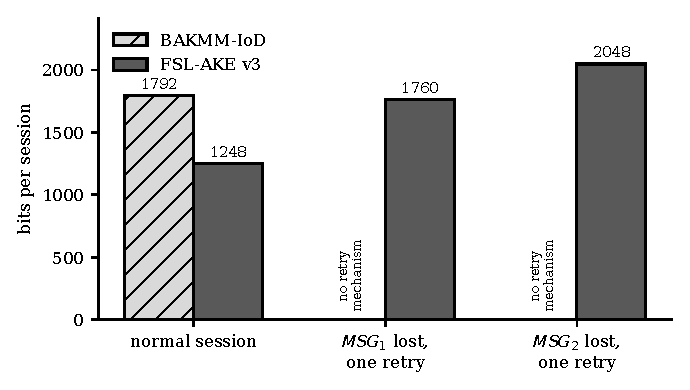
\includegraphics[width=0.62\textwidth]{figures/graph_comm_cases.pdf}
\caption{Communication per session in bits, field sizes of the BAKMM-IoD paper (Sec.~7.2), for a normal session and for one
retry after a lost $MSG_1$ or $MSG_2$ (\texttt{results/bench/paper\_count.json}; generated by
\texttt{paper/scripts/make\_graphs.py}).}
\label{fig:comm-cases}
\end{figure*}

\subsection{Storage}
\Cref{tab:storage} counts stored bits field by field. The drone stores \StoreDroneVthree\ bits against \StoreDroneBakmm\
(\PctStoreDrone\% lower), up to \StoreDroneVthreeMax\ while it waits for an answer. The server's own secrets take
\StoreOwnVthree\ bits against \StoreOwnBakmm. Per drone, however, the server stores \StoreServerVthree\ bits against
\StoreServerBakmm: BAKMM-IoD keeps $RID_{DE}$ and $MS$ in clear (the cause of F8), while v3 keeps encrypted indices, an
authenticated record and the retry ticket.
\begin{table*}[!htbp]
\centering
\footnotesize
\caption{Storage per entity, field by field, same counting rule for both schemes.}
\label{tab:storage}
\setlength{\tabcolsep}{3pt}
\begin{tabular}{p{1.6cm}lp{9.6cm}r}
\toprule
Entity & Scheme & Stored fields (bits) & Total \\
\midrule
drone & BAKMM-IoD & TID\_DE 160, RID\_DE 256, TC\_DE 256, MS\_DE-ES 256 & 928 \\
drone & v3 & TID 160, PID 96, K 256 & 512 \\
server per drone & BAKMM-IoD & TID\_DE 160, RID\_DE 256, MS\_DE-ES 256 & 672 \\
server per drone & v3 & I(TID): 2 AES blocks 256, I(PID): 1 AES block 128, record nonce nu 96, C = AEAD(K): ciphertext 256, C: tag 128, ticket index I(PID\_old): 1 AES block 128, ticket T: ciphertext of N2 160, ticket T: tag 128 & 1280 \\
server own & BAKMM-IoD & RID\_ES 256, TC\_ES 256 & 512 \\
server own & v3 & X\_ES 128 & 128 \\
\bottomrule
\end{tabular}
\end{table*}


\textbf{Growth with the number of drones.} The cost of one session is a constant number of operations per party in both
schemes ($O(1)$ per session), independent of the number of drones. Server storage grows linearly with the number $n$ of
registered drones: $\StoreServerVthree n + \StoreOwnVthree$ bits for v3 against $\StoreServerBakmm n + \StoreOwnBakmm$ bits
for BAKMM-IoD (\cref{fig:storage-n}). Our server implementation (\texttt{impl/server.py}) finds a record by its index $I(TID)$
or $I(PID)$ in a hash table (a Python dictionary), which takes expected constant time per lookup; the BAKMM-IoD paper does not
state its lookup structure.
\begin{figure}[!htbp]
\centering
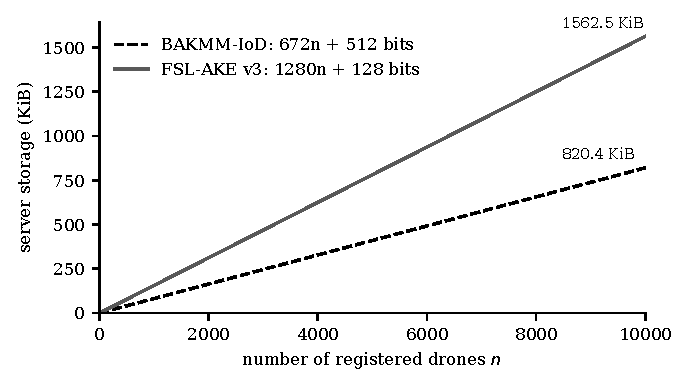
\includegraphics[width=\columnwidth]{figures/graph_storage_n.pdf}
\caption{Server storage against the number of registered drones $n$, from the field-by-field counts of \cref{tab:storage}
(per-drone bits $\times\, n$ + the server's own secrets); generated by \texttt{paper/scripts/make\_graphs.py}.}
\label{fig:storage-n}
\end{figure}

\subsection{Measured timings}
\Cref{tab:measured} gives the desktop measurements. The median drone time is \MeasDroneVthree\,ms for v3 and
\MeasDroneBakmm\,ms for BAKMM-IoD; the median server time is \MeasServerVthree\,ms for v3 and \MeasServerBakmm\,ms for
BAKMM-IoD, higher for v3. \Cref{fig:timing-box} shows the distribution of the \MeasRuns\ runs per party.
\begin{table}[!htbp]
\centering
\footnotesize
\caption{Measured time per session per party in ms, 1000 runs after 50 warm-up, on a desktop (13th Gen Intel(R) Core(TM) i7-1360P, Python 3.12.0, cryptography 46.0.7). These are desktop timings, not drone hardware. Computed from the per-run files \texttt{results/timing/raw\_*.csv} (run of 2026-10-19).}
\label{tab:measured}
\setlength{\tabcolsep}{3pt}
\begin{tabular}{llrrrrr}
\toprule
Scheme & Party & Mean & Median & Std dev & Min & Max \\
\midrule
BAKMM-IoD & drone & 0.0353 & 0.0349 & 0.0186 & 0.0224 & 0.5140 \\
BAKMM-IoD & server & 0.0351 & 0.0350 & 0.0132 & 0.0226 & 0.2245 \\
v3 & drone & 0.0232 & 0.0192 & 0.0315 & 0.0156 & 0.9774 \\
v3 & server & 0.0661 & 0.0578 & 0.0239 & 0.0478 & 0.3293 \\
\bottomrule
\end{tabular}
\end{table}

\begin{figure}[!htbp]
\centering
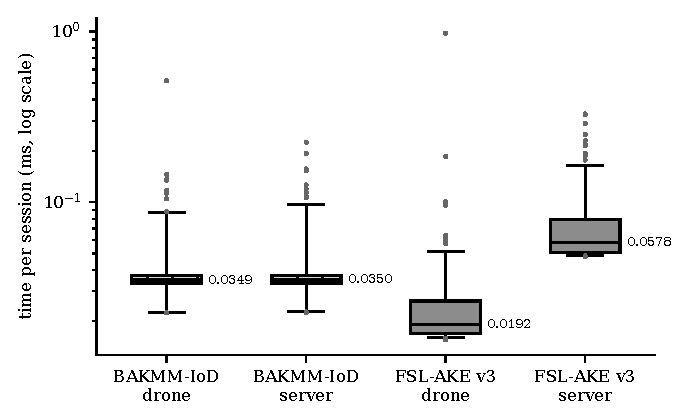
\includegraphics[width=\columnwidth]{figures/graph_timing_box.pdf}
\caption{Measured time per session and party, \MeasRuns\ runs after \MeasWarmup\ warm-up runs (\texttt{results/timing/raw\_*.csv});
boxes: quartiles, line and label: median, whiskers: 1st and 99th percentile, dots: runs outside them; log scale. Desktop
(\MeasCPU, Python \MeasPython, cryptography \MeasCrypto), not drone hardware. Generated by \texttt{paper/scripts/make\_graphs.py}.}
\label{fig:timing-box}
\end{figure}

\subsection{Summary}
\Cref{tab:final-cost} lists every quantity with its method and \cref{fig:charts} plots the main ones. v3 is lightweight on the
drone side and has lower communication in a normal session; it stores more per drone on the server, and its server time is
lower only if AES-GCM is at most \BreakEvenAEAD\,ms per operation: with the estimated AES-GCM time (estimate
\CostServerWithAEAD\,ms) and on measured desktop timings (\MeasServerVthree\ versus \MeasServerBakmm\,ms) it is higher.
\begin{table*}[!t]
\centering
\footnotesize
\caption{Cost summary, every quantity, including those where v3 is higher.}
\label{tab:final-cost}
\setlength{\tabcolsep}{3pt}
\begin{tabular}{p{3.6cm}rrrp{1.6cm}p{5.6cm}}
\toprule
Quantity & BAKMM-IoD & v3 & Diff. & Result & Method \\
\midrule
drone time, ms & 2.47 & 1.854 & -0.616 & \textbf{v3 lower} & paper method: our operation count x paper Table 7 (RPi 3) \\
server time, ms (paper primitives only) & 0.44 & 0.394 & -0.046 & \textbf{v3 lower} & paper method: our count x paper Table 6 \\
server time, ms (with estimated AES-GCM) & 0.44 & 0.96 & 0.52 & \textbf{v3 HIGHER} & paper method + AES-GCM time = desktop-measured ratio t(GCM)/t(SHA-256) x paper T\_h (estimate) \\
drone time, ms (measured median) & 0.0349 & 0.0192 & -0.0157 & \textbf{v3 lower} & measured: desktop (13th Gen Intel(R) Core(TM) i7-1360P), 1000 runs; not drone hardware \\
server time, ms (measured median) & 0.035 & 0.0578 & 0.0228 & \textbf{v3 HIGHER} & measured: desktop (13th Gen Intel(R) Core(TM) i7-1360P), 1000 runs \\
communication, bits per session & 1792 & 1248 & -544 & \textbf{v3 lower} & field lengths of the paper's Sec. 7.2 \\
drone storage, bits & 928 & 512 & -416 & \textbf{v3 lower} & field by field (paper\_count.json) \\
server storage per drone, bits & 672 & 1280 & 608 & \textbf{v3 HIGHER} & field by field \\
server own secrets, bits & 512 & 128 & -384 & \textbf{v3 lower} & field by field \\
\bottomrule
\end{tabular}
\end{table*}

\def\ChartDrone{(BAKMM-IoD,2.47) (v3,1.854)}
\def\ChartServer{(BAKMM-IoD,0.44) (v3,0.394)}
\def\ChartServerAEAD{(BAKMM-IoD,0.44) (v3,0.96)}
\def\ChartBits{(BAKMM-IoD,1792) (v3,1248)}
\def\ChartStoreDrone{(BAKMM-IoD,928) (v3,512)}
\def\ChartStoreServer{(BAKMM-IoD,672) (v3,1280)}

\begin{figure*}[!t]
\centering
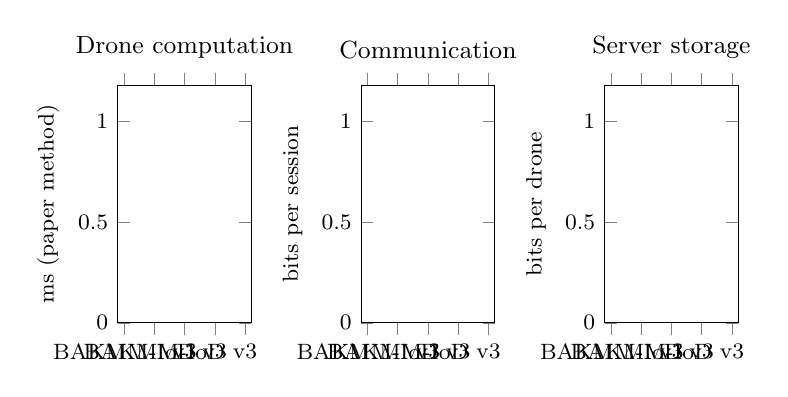
\begin{tikzpicture}
\begin{groupplot}[group style={group size=3 by 1, horizontal sep=1.4cm}, width=0.27\textwidth, height=4.6cm, ybar, /pgf/bar width=0.55cm, enlarge y limits={upper, value=0.18},
  symbolic x coords={BAKMM-IoD,v3}, xtick=data, ymin=0, enlarge x limits=0.6, nodes near coords, every node near coord/.append style={font=\footnotesize, /pgf/number format/precision=3, /pgf/number format/1000 sep={}},
  tick label style={font=\footnotesize}, label style={font=\footnotesize}, title style={font=\small}]
\nextgroupplot[title={Drone computation}, ylabel={ms (paper method)}] \addplot[fill=accent!70] coordinates {\ChartDrone};
\nextgroupplot[title={Communication}, ylabel={bits per session}] \addplot[fill=accent!70] coordinates {\ChartBits};
\nextgroupplot[title={Server storage}, ylabel={bits per drone}] \addplot[fill=black!35] coordinates {\ChartStoreServer};
\end{groupplot}
\end{tikzpicture}
\caption{BAKMM-IoD versus v3: drone computation (paper method), communication (normal session) and server storage per drone.
The first two panels, where v3 is lower, are drawn in blue; the third, where v3 is higher, in grey.}
\label{fig:charts}
\end{figure*}

\section{Discussion and limitations}\label{sec:discussion}

\textbf{No post-compromise security.} Every input of the next key except $K$ is public, so an attacker who learns $K$ once and
keeps listening computes every later $K$ and $SK$. Tamarin falsifies \texttt{pcs\_after\_K\_leak}. Recovery after a leak
\citep{cohngordon2016} would need fresh secret input such as a Diffie--Hellman step, which costs more drone computation.

\textbf{Captured drone (F6).} A drone's memory holds everything the server uses to prove itself, so an attacker holding it can
act as the server towards that drone (\texttt{captured\_drone\_accepts\_false\_server} falsified). Resisting this needs the
server to prove itself with a private key the drone does not hold, as in ephemeral--static Diffie--Hellman patterns
\citep{noise}.

\textbf{Database and $X_{ES}$ (F8 with $X_{ES}$).} An attacker holding both recovers $K$ and can act as the drone
(\texttt{drone\_impersonation\_with\_db\_and\_X} falsified). The database alone does not suffice
(\texttt{inj\_agree\_server} and \texttt{tid\_secrecy} verified with the database revealed; Tamarin, one session per pair).

\textbf{Linking a retry.} If the attacker drops $MSG_2$ for exactly one drone, that drone's retry receives a ticket while others
receive $MSG_2$, so the retry can be linked (equivalence falsified in the mixed scenario).

\textbf{Bounded proofs.} All drone--server Tamarin results are bounded to one session per pair (two for backward secrecy and
post-compromise security); the unbounded model ran out of memory. The BAKMM-IoD model with the same lemma text did not
terminate for \NumBakmmBaseDNT\ of \NumBakmmBaseLemmas\ lemmas, so most security rows cannot be compared lemma by lemma. Scyther has no state across runs, so it cannot express forward or backward secrecy or unlinkability. The ROR proof is a hand
proof.

\textbf{Scope of the comparison.} We compare v3 with BAKMM-IoD only; other IoD schemes were not re-implemented or re-verified,
so no ranking against them is claimed.

\textbf{Server storage.} Storing $K$ with plain two-block AES instead of AES-GCM would remove two AES-GCM operations per
session and part of the server storage, at the cost of record integrity, which is outside our threat model. We leave this
option as future work.

\textbf{Forward secrecy wording.} Forward secrecy here means: compromise of any party's long-term or current state does not
reveal session keys of sessions that completed before the compromise, a session having completed at a party when that party
erased its $SK$.

\section{Conclusion}\label{sec:conclusion}

We analysed BAKMM-IoD with Scyther and Tamarin and reported \NumFlawsConfirmed\ confirmed and \NumFlawsConditional\
conditional findings, from a published Scyther model that reaches no claim to missing forward secrecy, an alterable new
temporary identity, traceability on failed sessions and, under a stated condition, data-record replay. FSL-AKE v3 replaces XOR
masking by authenticated encryption, separates every hash by a label, erases and evolves its key at every session, repairs lost
messages with keyed one-time pseudonyms, confirms the key to the server and uses no timestamps. Tamarin verifies
\NumVthreeVerified\ of \NumVthreeLemmas\ drone--server lemmas within the stated bounds, the remaining ones being stated limits;
Scyther reports a proof of correctness for every explicit claim of the normal path; and a hand proof supports key
indistinguishability. With the BAKMM-IoD paper's timings, v3 lowers drone computation by \PctDrone\%, communication by
\PctBits\% and drone storage by \PctStoreDrone\%; it stores more per drone on the server (\StoreServerVthree\ versus
\StoreServerBakmm\ bits), and its server time is higher both with an estimated AES-GCM cost (estimate \CostServerWithAEAD\
versus \CostServerBakmm\,ms) and on desktop measurements (\MeasServerVthree\ versus \MeasServerBakmm\,ms). The last evidence
rerun of all packs (\texttt{results/evidence\_run.txt}) gave \EvItems\ items and \EvFail\ failures.


\section*{Data availability}
All models, scripts, raw tool outputs and evidence packs are in the artifact folder \texttt{fsl\_ake\_v2/v3/} of the
project repository: specification \texttt{spec/fsl\_ake\_v3.md}, Tamarin theories \texttt{tamarin/}, Scyther models
\texttt{scyther/}, reference implementation \texttt{impl/}, outputs \texttt{results/}, and \texttt{scripts/run\_all.sh} and
\texttt{scripts/run\_evidence.sh} to reproduce them. The tables of this paper are generated by
\texttt{paper/scripts/make\_tables.py}.

% STUB (to fill in): CRediT statement, printed from the \credit{} entries above
%\printcredits

\FloatBarrier
% Numbered references [1]. The CAS documentation names model1-num-names.bst (download from stmdocs); it is not in the
% CAS bundle. elsarticle-num-names.bst is Elsevier's equivalent numbered style and is included here.
\bibliographystyle{elsarticle-num-names}
\bibliography{refs}
\end{document}
